
\documentclass[twoside,12pt, a4paper]{report}

\usepackage[english]{babel}
\usepackage[utf8]{inputenc}
\usepackage{amsmath}
\usepackage{graphicx}
\setlength {\marginparwidth }{2.5cm}
\usepackage[left=3cm,right=3cm,top=2.5cm]{geometry}
\usepackage{float}
\usepackage{titlesec}
\usepackage{forest}
\usepackage{listings}
\usepackage{color}
\usepackage{eurosym}
\usepackage{ftnxtra}
\usepackage[fencedCode]{markdown}
\usepackage[T1]{fontenc}
\usepackage[colorinlistoftodos]{todonotes}
\usepackage{minted}
\usepackage{fnpos}
\usepackage[ruled,vlined]{algorithm2e}
\definecolor{dkgreen}{rgb}{0,0.6,0}
\definecolor{gray}{rgb}{0.5,0.5,0.5}
\definecolor{mauve}{rgb}{0.58,0,0.82}
\usepackage{hyperref}
\hypersetup{linktocpage}

\usepackage{booktabs} % Pour de meilleurs tableaux

\usepackage{longtable}
\providecommand{\keywords}[1]
{
  
  \textbf{Keywords---} #1
}

\urlstyle{same}

\lstset{
	aboveskip=3mm,
	belowskip=-2mm,
	backgroundcolor=\color{darkWhite},
	basicstyle=\footnotesize,
	breakatwhitespace=false,
	breaklines=true,
	captionpos=b,
	commentstyle=\color{red},
	deletekeywords={...},
	escapeinside={\%*}{*)},
	extendedchars=true,
	framexleftmargin=16pt,
	framextopmargin=3pt,
	framexbottommargin=6pt,
	frame=tb,
	keepspaces=true,
	keywordstyle=\color{blue},
	language=C,
	literate=
	{²}{{\textsuperscriptS}}1
	{⁴}{{\textsuperscript{4}}}1
	{⁶}{{\textsuperscript{6}}}1
	{⁸}{{\textsuperscript{8}}}1
	{€}{{\euro{}}}1
	{é}{{\'e}}1
	{è}{{\`{e}}}1
	{ê}{{\^{e}}}1
	{ë}{{\¨{e}}}1
	{É}{{\'{E}}}1
	{Ê}{{\^{E}}}1
	{û}{{\^{u}}}1
	{ù}{{\`{u}}}1
	{â}{{\^{a}}}1
	{à}{{\`{a}}}1
	{á}{{\'{a}}}1
	{ã}{{\~{a}}}1
	{Á}{{\'{A}}}1
	{Â}{{\^{A}}}1
	{Ã}{{\~{A}}}1
	{ç}{{\c{c}}}1
	{Ç}{{\c{C}}}1
	{õ}{{\~{o}}}1
	{ó}{{\'{o}}}1
	{ô}{{\^{o}}}1
	{Õ}{{\~{O}}}1
	{Ó}{{\'{O}}}1
	{Ô}{{\^{O}}}1
	{î}{{\^{i}}}1
	{Î}{{\^{I}}}1
	{í}{{\'{i}}}1
	{Í}{{\~{Í}}}1,
	morekeywords={*,...},
	numbers=left,
	numbersep=10pt,
	numberstyle=\tiny\color{black},
	rulecolor=\color{black},
	showspaces=false,
	showstringspaces=false,
	showtabs=false,
	stepnumber=1,
	stringstyle=\color{gray},
	tabsize=4,
	title=\lstname,
}

\lstdefinestyle{frameStyle}{
	basicstyle=\footnotesize,
	numbers=left,
	numbersep=20pt,
	numberstyle=\tiny\color{black}
}



\setcounter{secnumdepth}{3}

%\usepackage{biblatex} %Imports biblatex package
\usepackage[
    backend=biber,
    style=numeric,
    sortlocale=fr_FR,
    natbib=true,
    url=false,
    doi=true,
    eprint=false
]{biblatex}
\addbibresource{references.bib} %Import the bibliography file



\definecolor{darkWhite}{rgb}{0.94,0.94,0.94}




\titleformat{\paragraph}
{\normalfont\normalsize\bfseries}{\theparagraph}{1em}{}
\titlespacing*{\paragraph}
{0pt}{3.25ex plus 1ex minus .2ex}{1.5ex plus .2ex}

\begin{document}
\begin{titlepage}
\newcommand{\HRule}{\rule{\linewidth}{0.5mm}} % Defines a new command for the horizontal lines, change thickness here

\center % Center everything on the page
 
%----------------------------------------------------------------------------------------
%	HEADING SECTIONS
%----------------------------------------------------------------------------------------

\textsc{\LARGE Université Libre de Bruxelles}\\[1.5cm] % Name of your university/college
\textsc{\Large }\\[0.5cm] % Major heading such as course name

%----------------------------------------------------------------------------------------
%	TITLE SECTION
%----------------------------------------------------------------------------------------

\HRule \\[0.4cm]
{ \huge Line Simplification Algorithm \bfseries }\\[0.4cm] % Title of your document
\HRule \\[1.2cm]
 
%----------------------------------------------------------------------------------------
%	AUTHOR SECTION
%----------------------------------------------------------------------------------------

\begin{minipage}{0.4\textwidth}
\begin{flushleft} \large
\emph{Authors:}\\
Soufiane \textsc{AJOUAOU}\\  000459811\\


\end{flushleft}
\end{minipage}
~
\begin{minipage}{0.5\textwidth}
\begin{flushright} 
\emph{Supervisors:} \\
 \textsc{Esteban Zimanyi}\\


\end{flushright}
\end{minipage}\\[2cm]

% If you don't want a supervisor, uncomment the two lines below and remove the section above
%\Large \emph{Author:}\\
%John \textsc{Smith}\\[3cm] % Your name

%----------------------------------------------------------------------------------------
%	DATE SECTION
%----------------------------------------------------------------------------------------

{\large \today}\\[1cm] % Date, change the \today to a set date if you want to be precise

%----------------------------------------------------------------------------------------
%	LOGO SECTION
%----------------------------------------------------------------------------------------


\includegraphics[width=3.3cm, height=3.3cm]{sceau-a-quadri.jpg}%% Include a department/university logo - this will require the graphicx package
 
%----------------------------------------------------------------------------------------

\end{titlepage}


\section*{Abstract}
With the increasing use of real-time geospatial data, particularly for GPS navigation and dynamic geospatial data analysis applications, line simplification is essential for efficiently representing complex and voluminous data. The ability to process this data quickly and accurately is crucial to meet the needs of modern applications.

However, simplifying trajectories in a real-time processing environment poses significant challenges. Existing algorithms, such as Douglas-Peucker and Visvalingam-Whyatt, are not optimized for continuous data streams, limiting their effectiveness in scenarios where data continuously arrives and requires dynamic adaptation.

To address this need, this thesis proposes the SQUISH-E algorithm, designed to simplify trajectories in real time while minimizing synchronized Euclidean distance (SED) error. The algorithm uses a priority queue structure to maintain a simplified approximation of trajectories, enabling efficient data compression without sacrificing spatial accuracy. This solution is integrated into the POSTGIS and MobilityDB environments, allowing for practical and performant implementation in geospatial database systems.
[00:41]
The advantages of this solution are numerous. The results show that the SQUISH-E algorithm significantly improves execution time compared to traditional implementations, particularly due to its efficiency in C. Additionally, the algorithm maintains high precision in trajectory simplification, as demonstrated by Hausdorff distance, Frechet distance, and Dynamic Time Warping measurements. Thus, the SQUISH-E algorithm substantially contributes to solving real-time line simplification problems, making geospatial data processing applications faster and more accurate.


\vspace{10pt}

%TC:ignore
\keywords{Line Simplification Algorithm, MobilityDB, Trajectory compression, Streaming algorithm, Trajectory reduction}

\newpage

\section*{Acknowledgements}
Je souhaite exprimer ma sincère reconnaissance et ma gratitude à l'égard de tous ceux qui ont participé à la concrétisation de ce projet. Ce projet s'est avéré être à la fois difficile et prolongé, et je tiens à exprimer ma gratitude envers celui qui m'a aidé à l'accomplir et qui m'a soutenu tout au long de ma vie, même avant ma naissance. Sans lui, rien ne pourrait se produire, pas même la chute d'une goutte de pluie. Je tiens également à exprimer ma gratitude envers Esteban Zimanyi, qui a fait preuve de grande patience et qui a assuré une supervision remarquable, malgré les divers obstacles et les retards survenus lors de la rédaction de cette thèse. Je tiens également à exprimer ma gratitude envers Mahmoud SAKR et Gilles DEJAEGERE pour leur dévouement, leur intérêt et leurs conseils avisés, qui m'ont été précieux pour trouver des idées pour ma thèse. Mes parents et ma famille m'ont non seulement soutenu, mais m'ont également aidé à découvrir une autre facette du monde, différente de ce que l'on peut voir à travers un écran d'ordinateur. De la même manière que mes amis m'ont aidé à trouver des ressources et à rédiger ce travail. Je tiens également à exprimer ma gratitude envers l'ULB pour avoir proposé ce master en informatique et la Belgique pour le soutien qu'elle m'a accordé. Je vous souhaite tout le bonheur possible pour votre vie et une issue heureuse pour tout ce que vous entreprenez. Je suis également reconnaissant envers la source de tout bienfait et je ne serai jamais assez reconnaissant pour tous les privilèges dans lesquels je suis baigné. 
\newpage


\tableofcontents

\listoffigures
\listoftables
\lstlistoflistings




\chapter{Introduction}


In cartography, the need to simplify complex geographical data for clear and efficient representation is becoming increasingly important. The rise of automated cartography driven by computer technologies has heightened the demand for efficient algorithms, especially in the areas of feature extraction and simplification.\\


This master thesis aims to contribute to the study of cartographic representation techniques, with a central emphasis on the utilization of POSTGIS and MobilityDB \cite{zimanyi2019mobilitydb}, by exploring solutions for real-time processing of trajectories. Indeed dynamic adaptability is crucial in modern applications such as GPS navigation, real-time geospatial data analysis, and the constant monitoring of geospatial data streams, all of which are integral to the POSTGIS and MobilityDB ecosystems.\\



In this study, our primary aim will be to simplify line representations of mobility data within the environment of POSTGIS and MobilityDB. This involves the processing of an ordered set of n+1 points in a plane, delineating a polygonal path composed of line segments, and deriving a simplified path with fewer segments while preserving the fundamental attributes of the initial path. Our study stands out for its focus on the real-time nature of the data, which aligns well with the principles and capabilities of POSTGIS and MobilityDB.\\




An underlying assumption for this work is the simplicity of the provided path, with an absence of self-intersections. The presence of self-intersections in cartographic data often indicates issues related to digitization errors. While our goal is to keep the resulting approximation simple, the issue of computational feasibility within the POSTGIS and MobilityDB environment is a key consideration.\\




The idea of effectively representing data involves several aspects, such as keeping the original and simplified paths close, minimizing the area between them, incorporating critical points from the original path into the simplified one, and optimizing various measures of curve discrepancy. These aspects represent challenges to overcome for an effective real-time trajectory compression algorithm because of the limited information available about the path being processed.\\



\iffalse
\subsection{Definitions and Key Concepts}
In this subsection, we will establish a foundational understanding of key terms and concepts central to the research presented in this thesis. These definitions are essential for comprehending the context and significance of the study.

\subsubsection{Moving Objects}

Moving objects refer to entities or points that continuously change their positions in a given space over time. In the context of this research, moving objects represent dynamic or mobile assets, including vehicles, individuals, or any entities with ever-changing spatial coordinates. Understanding the behavior of moving objects is fundamental for the stream algorithm proposed in this study.

\subsubsection{Stream Data}

Stream data pertains to the continuous and real-time flow of data that arrives sequentially. In the context of this research, stream data represents the dynamic nature of the information being processed. Stream data includes data points, such as the changing positions of moving objects, which are received and processed as they become available over time.


\subsubsection{Polygonal Path}

A polygonal path is a sequence of line segments connected end-to-end, forming a coherent trajectory or route. In the context of this research, a polygonal path represents the course taken by moving objects, represented as a series of line segments, which is the primary focus of the stream algorithm for simplification.


\subsubsection{Restricted Version}

A restricted version in this context signifies a specialized or limited form of an algorithm or problem. It is tailored to accommodate specific constraints or requirements pertinent to the application. For example, a restricted version of a line simplification algorithm may be designed to address particular limitations associated with moving objects and streaming data.



\subsubsection{Function Error}

Function error indicates the degree of discrepancy between an ideal or reference function and an approximation or simplified representation. In the context of line simplification, it quantifies the degree to which the simplified line retains the essential characteristics of the original polygonal path.

\subsubsection{Fréchet Distance}

The Fréchet distance is a distance metric that quantifies the similarity between two curves or paths. It measures the likeness between the original polygonal path and a simplified path by considering the minimum separation distance between a moving object on each path as they traverse from start to end.


\subsubsection{The Hausdorff Distance}

The Hausdorff distance is another distance metric used to measure the similarity or dissimilarity between two sets or paths. It calculates the maximum distance from each point in one set to the nearest point in the other set, providing a measure of the dissimilarity between paths.


\subsubsection{Convex Paths}

Convex paths represent polygonal paths with the property that any line segment connecting two points lies entirely within the convex hull of the points. Convex paths exhibit certain geometric properties that can be advantageous in the context of simplification algorithms.

\subsubsection{XY-Monotone Paths}

An XY-monotone path is a polygonal path with the characteristic of being monotonic in both the x and y directions. Such paths move in one direction along the x and y axes without backtracking.

\subsubsection{General Paths}

General paths encompass polygonal paths without specific constraints on their geometry. They may exhibit complex shapes, including non-monotonic behavior, sharp turns, and diverse geometric characteristics.

\fi


\chapter{State of the Art}
This section will present a review of the literature on line simplification algorithms, stream processing algorithms and introduce several notions related to the subject of this master thesis.


\section{Error Metrics}

In this section we will explain how to compare a trajectory with its simple counterpart in detail. In this study, a trajectory is represented as a polyline P, which is made up of a series of points  $\{p_{1},..., p_{n}\}$, where the points pi are made up of the longitude, latitude, and sample time-stamp, Xi, Yi, and ti, respectively. Approximation A, which is a subset of P, the polyline of the original trajectory, is the name given to the simplified version of a trajectory \cite{van2017extensive}. Moreover, the original trajectory's p1 and pn must be included in Approximation A.
In the thesis we will focus on a spatial metrics in order to compare the trajectory and its simple version.

\subsection{Hausdorff Distance}


One simple similarity measure for trajectories is the Hausdorff distance. It is a very
general similarity measure that can be used for any two point sets. If we have two
sets of points P and Q, such as two trajectories if we treat them as polygonal curves
and disregard the timestamps, the directed Hausdorff distance from P to Q is equal
to the Euclidean distance between the point in P that is furthest from any point in
Q, and the point in Q that is closest to that point \cite{kerkhof2022algorithmic}. Written formally, we get:

$$\overrightarrow{\mathrm{H}}(P, Q)=\max _{p \in P} \min _{q \in Q} \| p-q \| $$

The undirected Hausdorff distance, also just called the Hausdorff distance, is then
the maximum of the directed distances in both directions.

$$\mathrm{H}(P, Q)=\max \{\overrightarrow{\mathrm{H}}(P, Q), \overrightarrow{\mathrm{H}}(Q, P)\} $$


\subsection{Frechet Distance}


Another trajectory similarity measure that we use often is the Fréchet distance. It
is based on the principle that similar polygonal curves should not just be close in
space, but there should also exist some parametrization of the curves such that if
we traverse both simultaneously we should remain close at all times \cite{kerkhof2022algorithmic}. Closeness
here is defined as having small Euclidean distance. The trajectories are treated as
polygonal curves and the timestamps are not taken into account. For polygonal
curves/trajectories P and Q, with P and Q probes respectively, the Fréchet distance
is defined as:

$$\mathrm{F}(P, Q)=\inf _{(\sigma, \theta)} \max _{j:[0,1]}\|P(\sigma(j))-Q(\theta(j))\| $$

where  $ \sigma $   and $ \theta  $  are continuous non-decreasing functions from [0, 1] to the real intervals [1, n] and [1,m], respectively.
This is often explained with the following analogy: Suppose someone is walking
their dog. P is the path the owner takes, and Q is the path of the dog. The owner
and dog can change their speed at will, but they cannot go backwards on the path.
The Fréchet distance is then the shortest possible length the dog’s leash can have
for this walk to be possible.
The weak Fréchet distance is similar, but the constraint is dropped that  $ \sigma $    and $ \theta $
are non-decreasing. Going back to the man-walking-dog analogy this means the
man and dog can freely move backwards and forwards over their path if this results
in a shorter leash being needed. The weak Fréchet distance between curves thus
gives a lower bound for the (strong) Fréchet distance.
The discrete Fréchet distance is a variant where  $ \sigma $    and $ \theta $   are discrete functions
from {0,..., k} to {1,..., n} and {1,...,m} with the property that
$0 \leq \sigma (i+1)-\sigma    (i) \leq 1$
and $0 \leq  \theta   (i + 1)-\theta   (i) \leq 1$. This has been explained as someone walking a pet frog,
where instead of walking along edges of the polygonal curve, the owner and frog can
only hop from vertex to vertex. The discrete Fréchet distance between two curves
gives an upper bound on their (continuous) Fréchet distance.
As you might expect, computing the exact Fréchet distance between two curves
is not completely straightforward. Alt and Godau \cite{AltGodau} described an approach for
computing this distance. They de $ \sigma $   ne an algorithm for solving a decision variant of
the problem of computing the distance. This algorithm can answer if the Fréchet
distance between two curves is at most some value $ \delta $ . Then they use a technique
called parametric search to  $ \sigma $   nd the minimum value of $ \delta $ .
Their decision algorithm works by constructing what is called a free space diagram
for a value for $ \delta $ .
It consists of a grid of $   (n - 1)  \times  (m - 1)$ cells, where each cell corresponds to a pair
of line segments, one from P and one fromQ. Each column of cells corresponds to an
edge of P and each row corresponds to an edge of Q. For example, the point (2.6, 3.5)
in a free space diagram corresponds to the probe gotten by linearly interpolating
between P’s second and third probes with a $ \lambda $  of 0.6, and the probe gotten by linearly
interpolating between Q’s third and fourth probes with a $ \lambda $  of 0.5. Each cell is divided
into free space and forbidden space. If the Euclidean distance between the curves at a
point is less than or equal to $ \delta $ , the point is in the free space. If the distance is greater
than $ \delta $ , the point lies in the forbidden space. See Figure \ref{fig:fsd}.


\begin{figure}[!h]
    \centering
    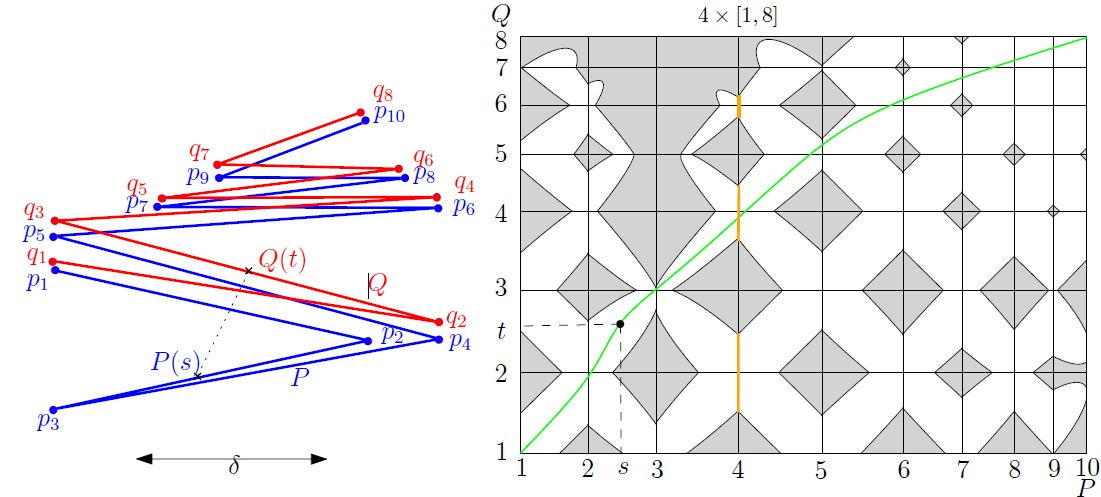
\includegraphics[width=1.0\linewidth]{figures/Figure.jpg}
    \caption[Free space diagram of polygonal curves P and Q for a given $ \delta $]{Enter Two polygonal curves P (in blue) and Q (in red), and their free space
    diagram for the chosen value of  $ \delta $. The free space is shown in white and the forbidden
    space is shown in gray. Each cell of the FSD corresponds to the combination of
    one edge of P and one edge of Q. (s, t) is a free point in the diagram, lying on a
    reachable path in the free space. One green spot is marked in both the FSD and on
    the associated spots on P and Q. A x- and y- monotone path contained in the free
    space from (1, 1) to (8, 10), shown in green, corresponds to parametrizations of P and
    Q realizing a Fréchet distance of at most  $ \delta $ \cite{kerkhof2022algorithmic}.}
    \label{fig:fsd}
\end{figure}
\vspace{1cm}
Now, an x- and y-monotone path from the point (1, 1) to (n,m) entirely through
the free space corresponds to parametrizations of P and Q such that the distance
between the two is at most $ \delta $  at any time, i.e. the Fréchet distance is at most $ \delta $ .
For additional details we refer to the paper by Alt and Godau \cite{AltGodau}.

\subsection{Dynamic Time Warping Distance}
%TO DO% Describe the dynamic time warping distance similarities
Dynamic Time Warping (DTW) is a techniques to find the optimal alignment between two sequences in same time. The DTW distance take into account the time dimension. This distance can be expressed as the minimum cost of a warping path p between X and Y where X and Y are two sequences (time-dependant). \cite{muller2007dynamic}

\section{Line Simplification Algorithm}
Line simplification deals with the simplification of arbitrary lines, which can be straight or curved. The goal is to reduce the complexity of lines while still ensuring that the simplified representation captures the main features of the original lines. This algorithm address the problem of Line simplification this problem who is relevant for GPU computing and Spatial Data processing

\subsection{Douglas-Peucker Algorithm}
The Douglas-Peucker algorithm  \cite{douglas1973algorithms} \cite{hershberger1994n} takes a polyline
P a sequence of points $\{p_{1},..., p_{n}\}$ , and a user defined
allowed spatial error, $\varepsilon$ > 0. The algorithm builds an
approximation polyline $P'$ , initially consisting of $p_{1}$ and
$p_{n}$. It continues adding the point pi out of the original
polyline that has the largest shortest-euclideandistance
to $P'$ until that distance is smaller than $\varepsilon$ as
demonstrated in Figure \ref{fig:dgpk}.

\begin{figure}[!h]
    \centering
    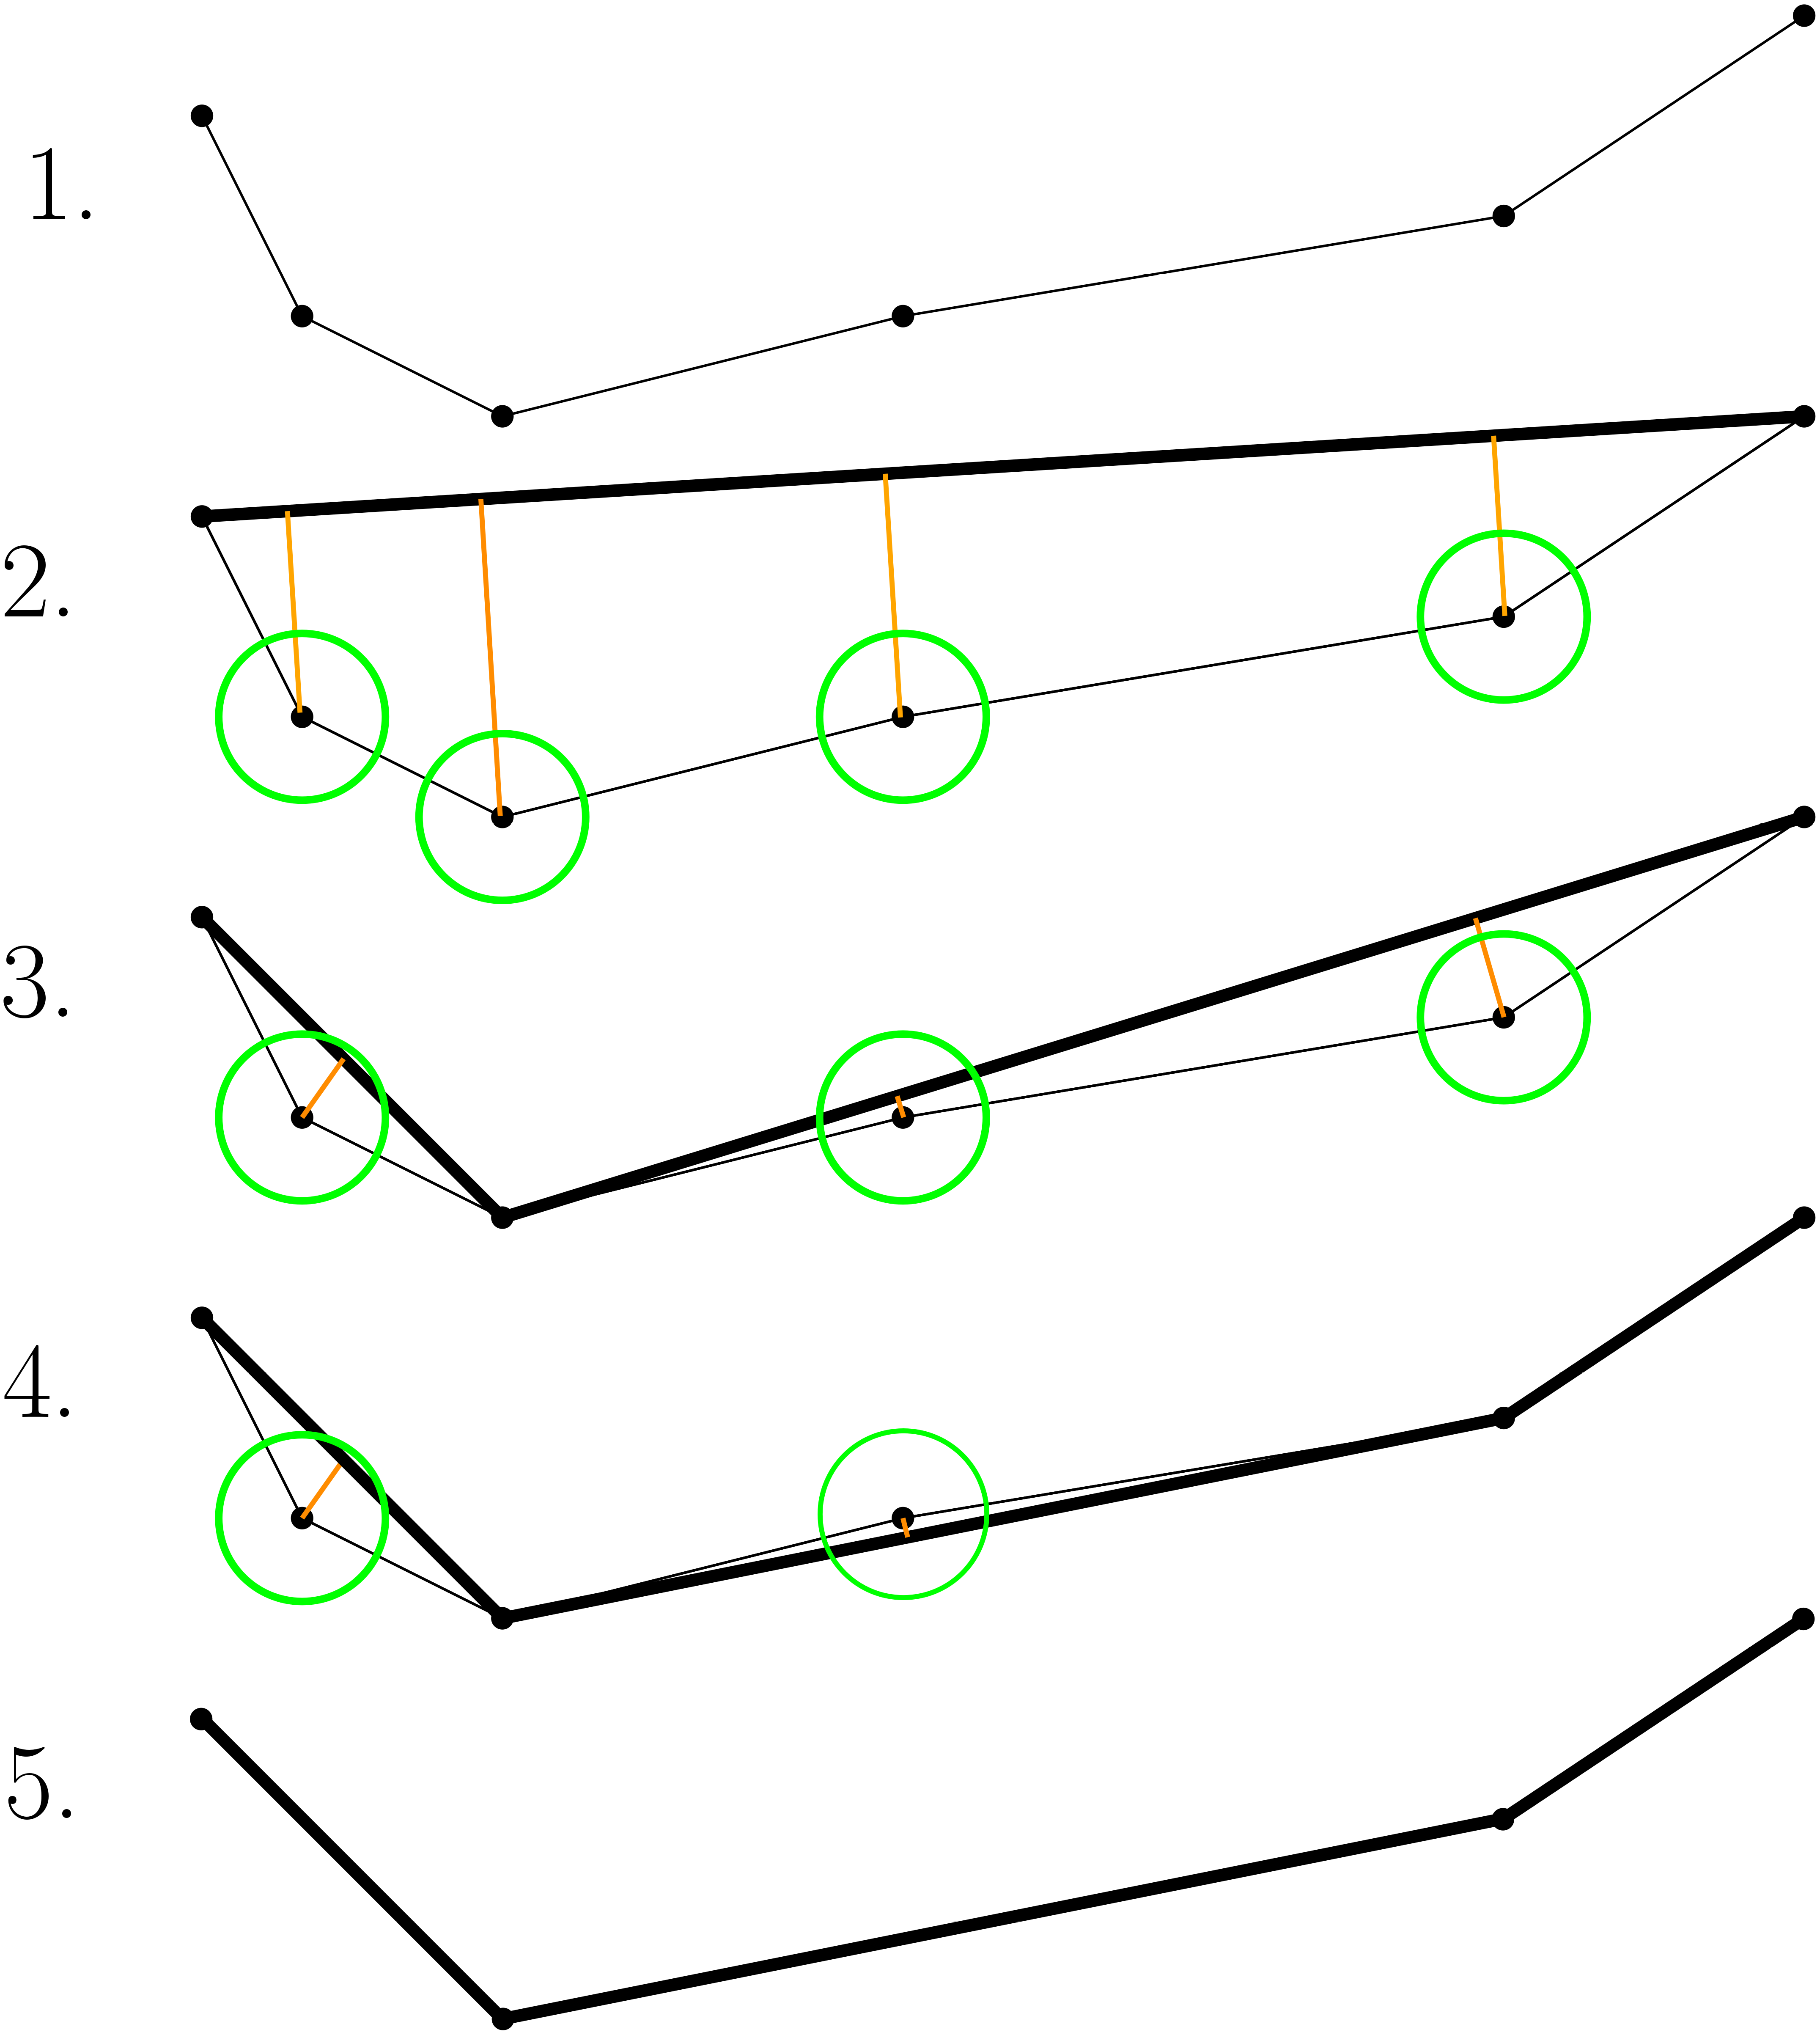
\includegraphics[width=0.5\linewidth]{figures/dgpk.png}
    \caption{Illustration of how the Douglas-Peucker algorithm
    iteratively simplifies a line. The allowed spatial
    error  $\varepsilon$  is depicted with green circles \cite{van2017extensive}. }
    \label{fig:dgpk}
\end{figure}

\subsection{Visvalingam-Whyatt Algorithm}

The Visvalingam-Whyatt algorithm \cite{doi:10.1179/000870493786962263} uses the concept
of ‘effective area’, which is the area of the triangle
formed by a point and its two neighbors. The algorithm
takes a polyline P a sequence of points $\{p_{1},..., p_{n}\}$, and
a user defined allowed spatial displacement error, $\varepsilon$ > 0.
For every set of three consecutive points $\{p_{i-1},p_{i},p_{i+1}\}$
a triangle is formed with its surface being the ‘effective area’. Iteratively point $p_{i}$ is dropped that results in
the least areal displacement to form an approximation
as illustrated in Figure \ref{fig:visv}. This process halts when the
‘effective area’ is larger than $\varepsilon$.

\begin{figure}[!h]
    \centering
    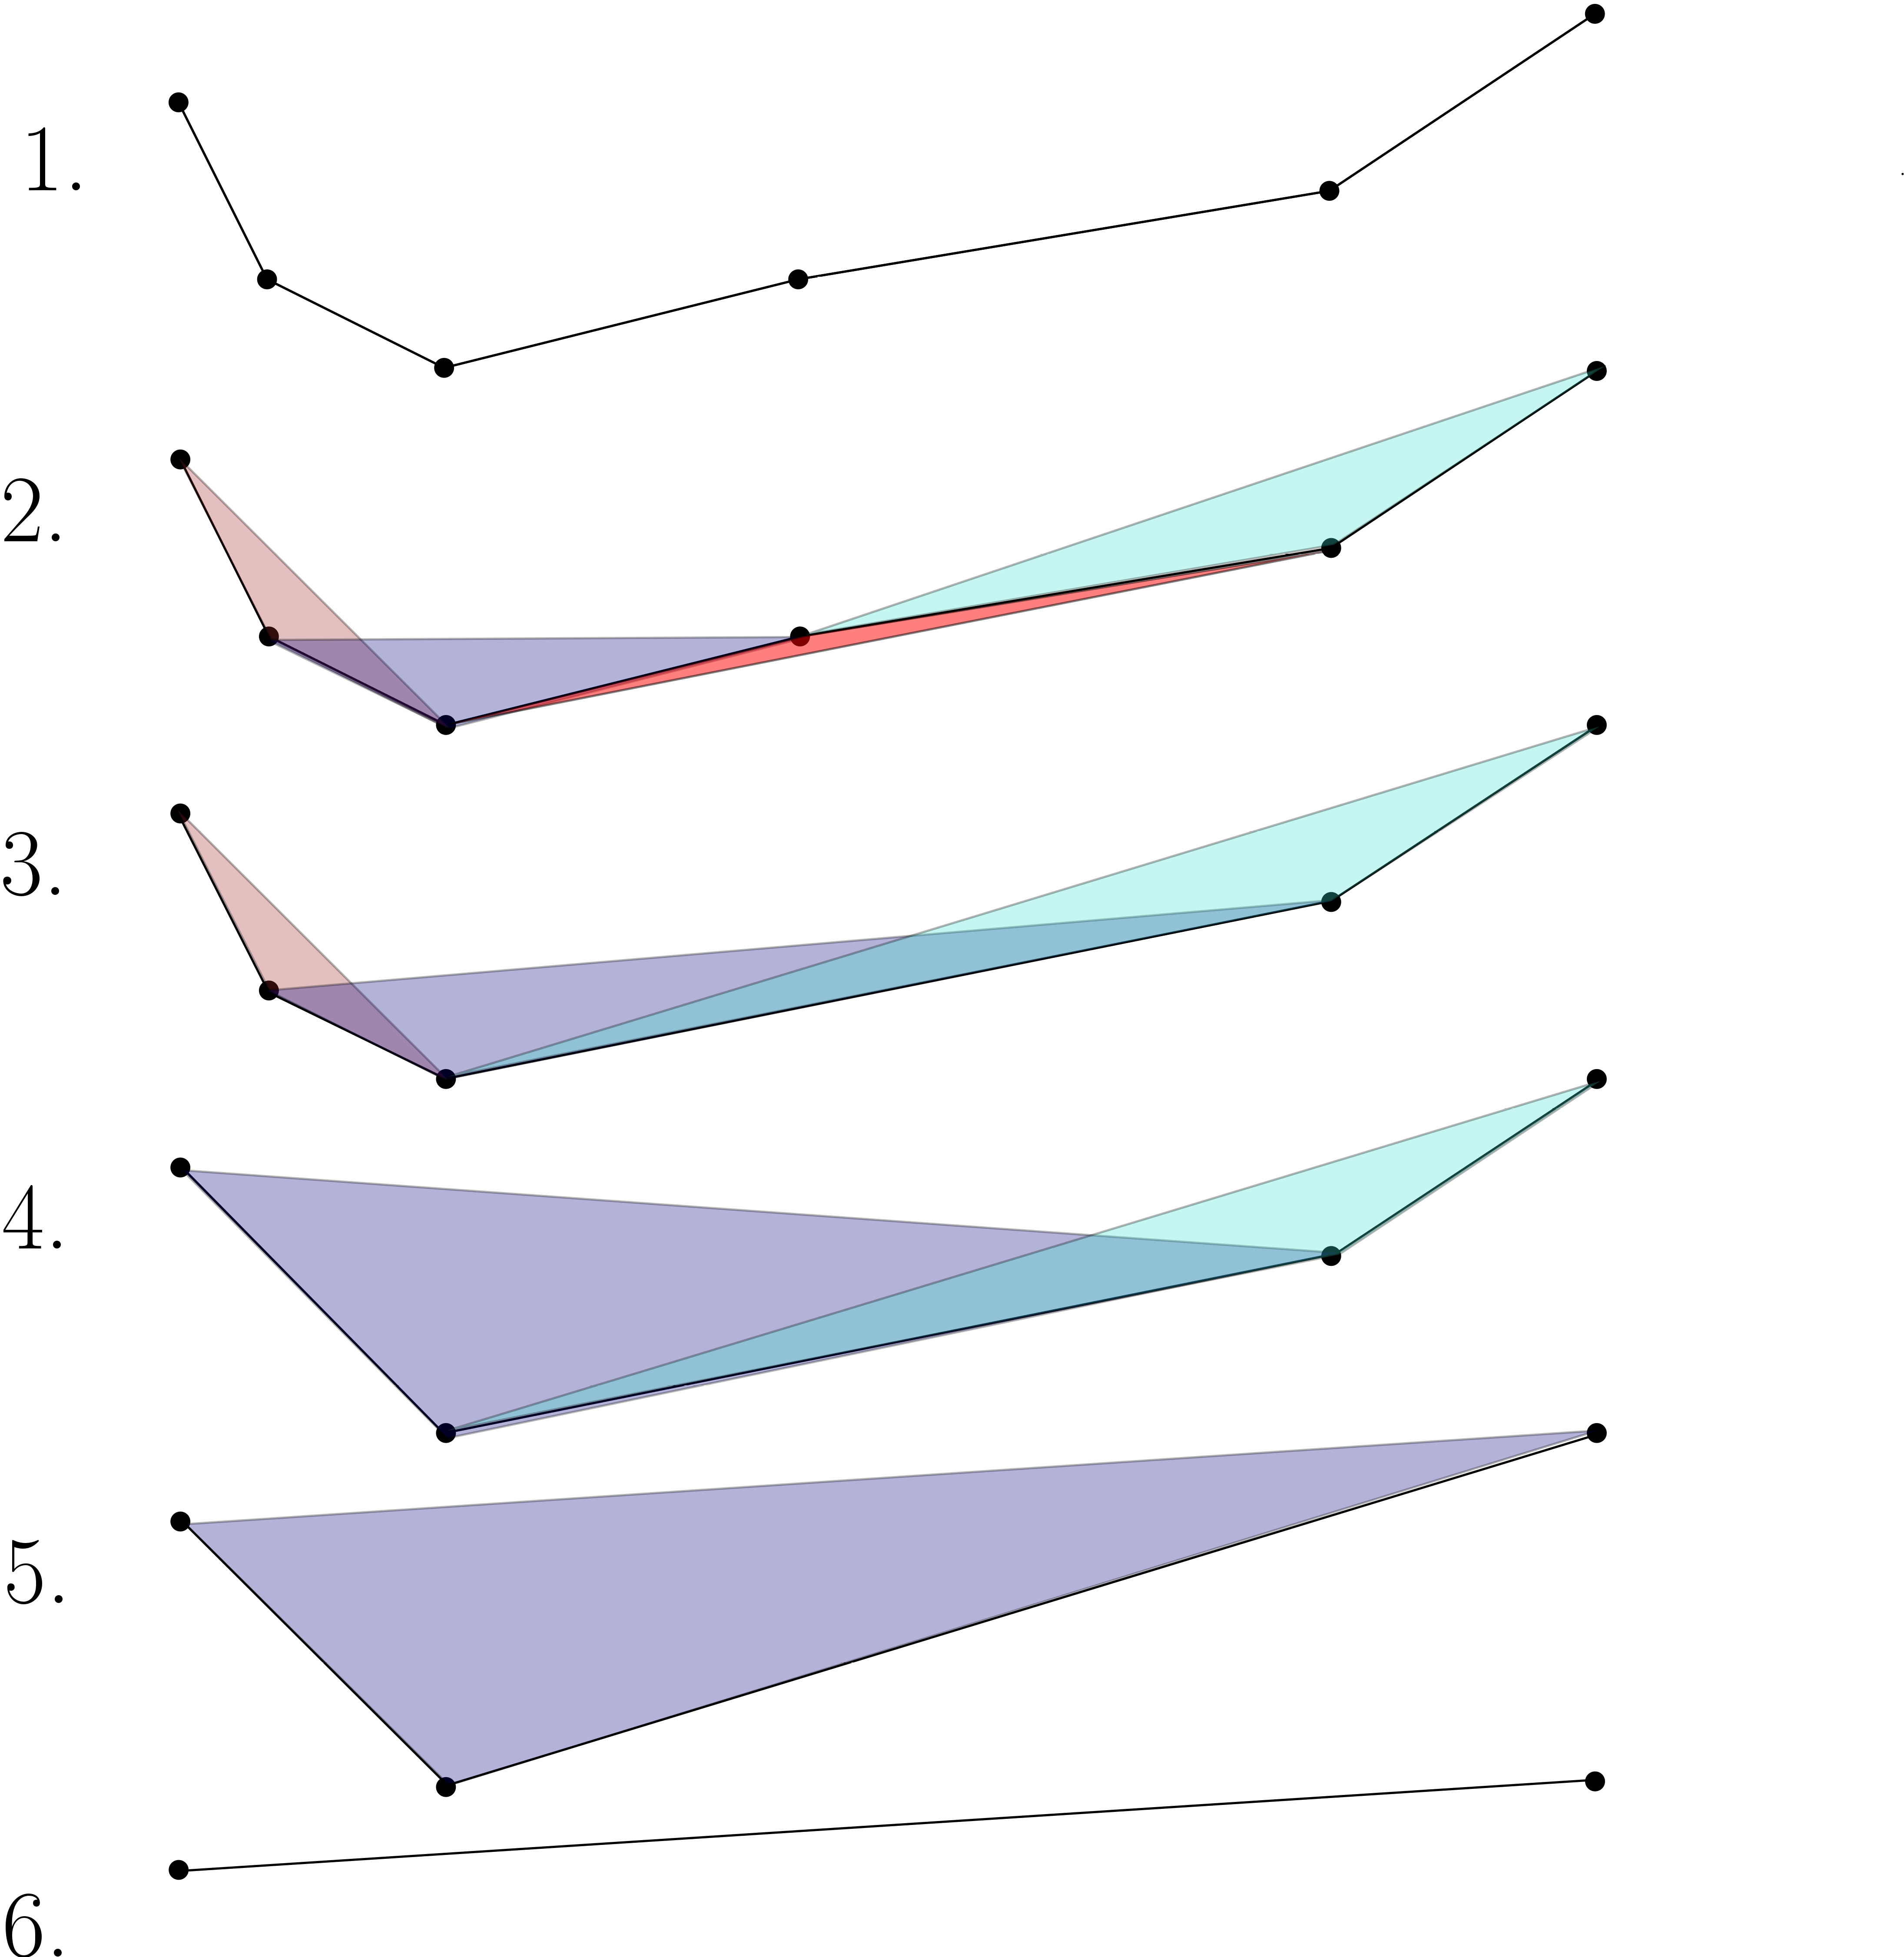
\includegraphics[width=0.5\linewidth]{figures/visv.png}
    \caption{Illustration of how the Visvalingam-Whyatt
    algorithm iteratively simplifies the line \cite{van2017extensive}.}
    \label{fig:visv}
\end{figure}
\newpage

\subsection{Imai-Iri}
The basis of the Imai-Iri algorithm \cite{IMAI198631} lies in the construction
of an unweighted directed acyclic graph G.
This graph is constructed by connecting all combinations
of two points that would create an allowed shortcut.
A breadth-first search is done on this graph to
compute the shortest path connecting the first and last
point, resulting in the approximation.
This algorithm takes a polyline P a sequence of
points $\{p_{1},..., p_{n}\}$, and a user defined allowed spatial
error, $\varepsilon $ > 0. For each combination of two points ($p_{i}$ and $p_{j}$) it checks if a line between them intersects all
circles with radius $\varepsilon $ that center on the points that lie{\tiny {\tiny }}
between them $\{p_{x} > p_{i},p_{x} < p_{j}\}$. When this is the
case, the line $p_{i}p_{j}$ is an allowed shortcut and is added
to the graph G, see Figure \ref{fig:imai}. After all allowed shortcuts
are added to graph G, breadth-first search is done
to find the shortest path through the graph from $p_{1}$ to $p_{n}$.

\begin{figure}[!h]
    \centering
    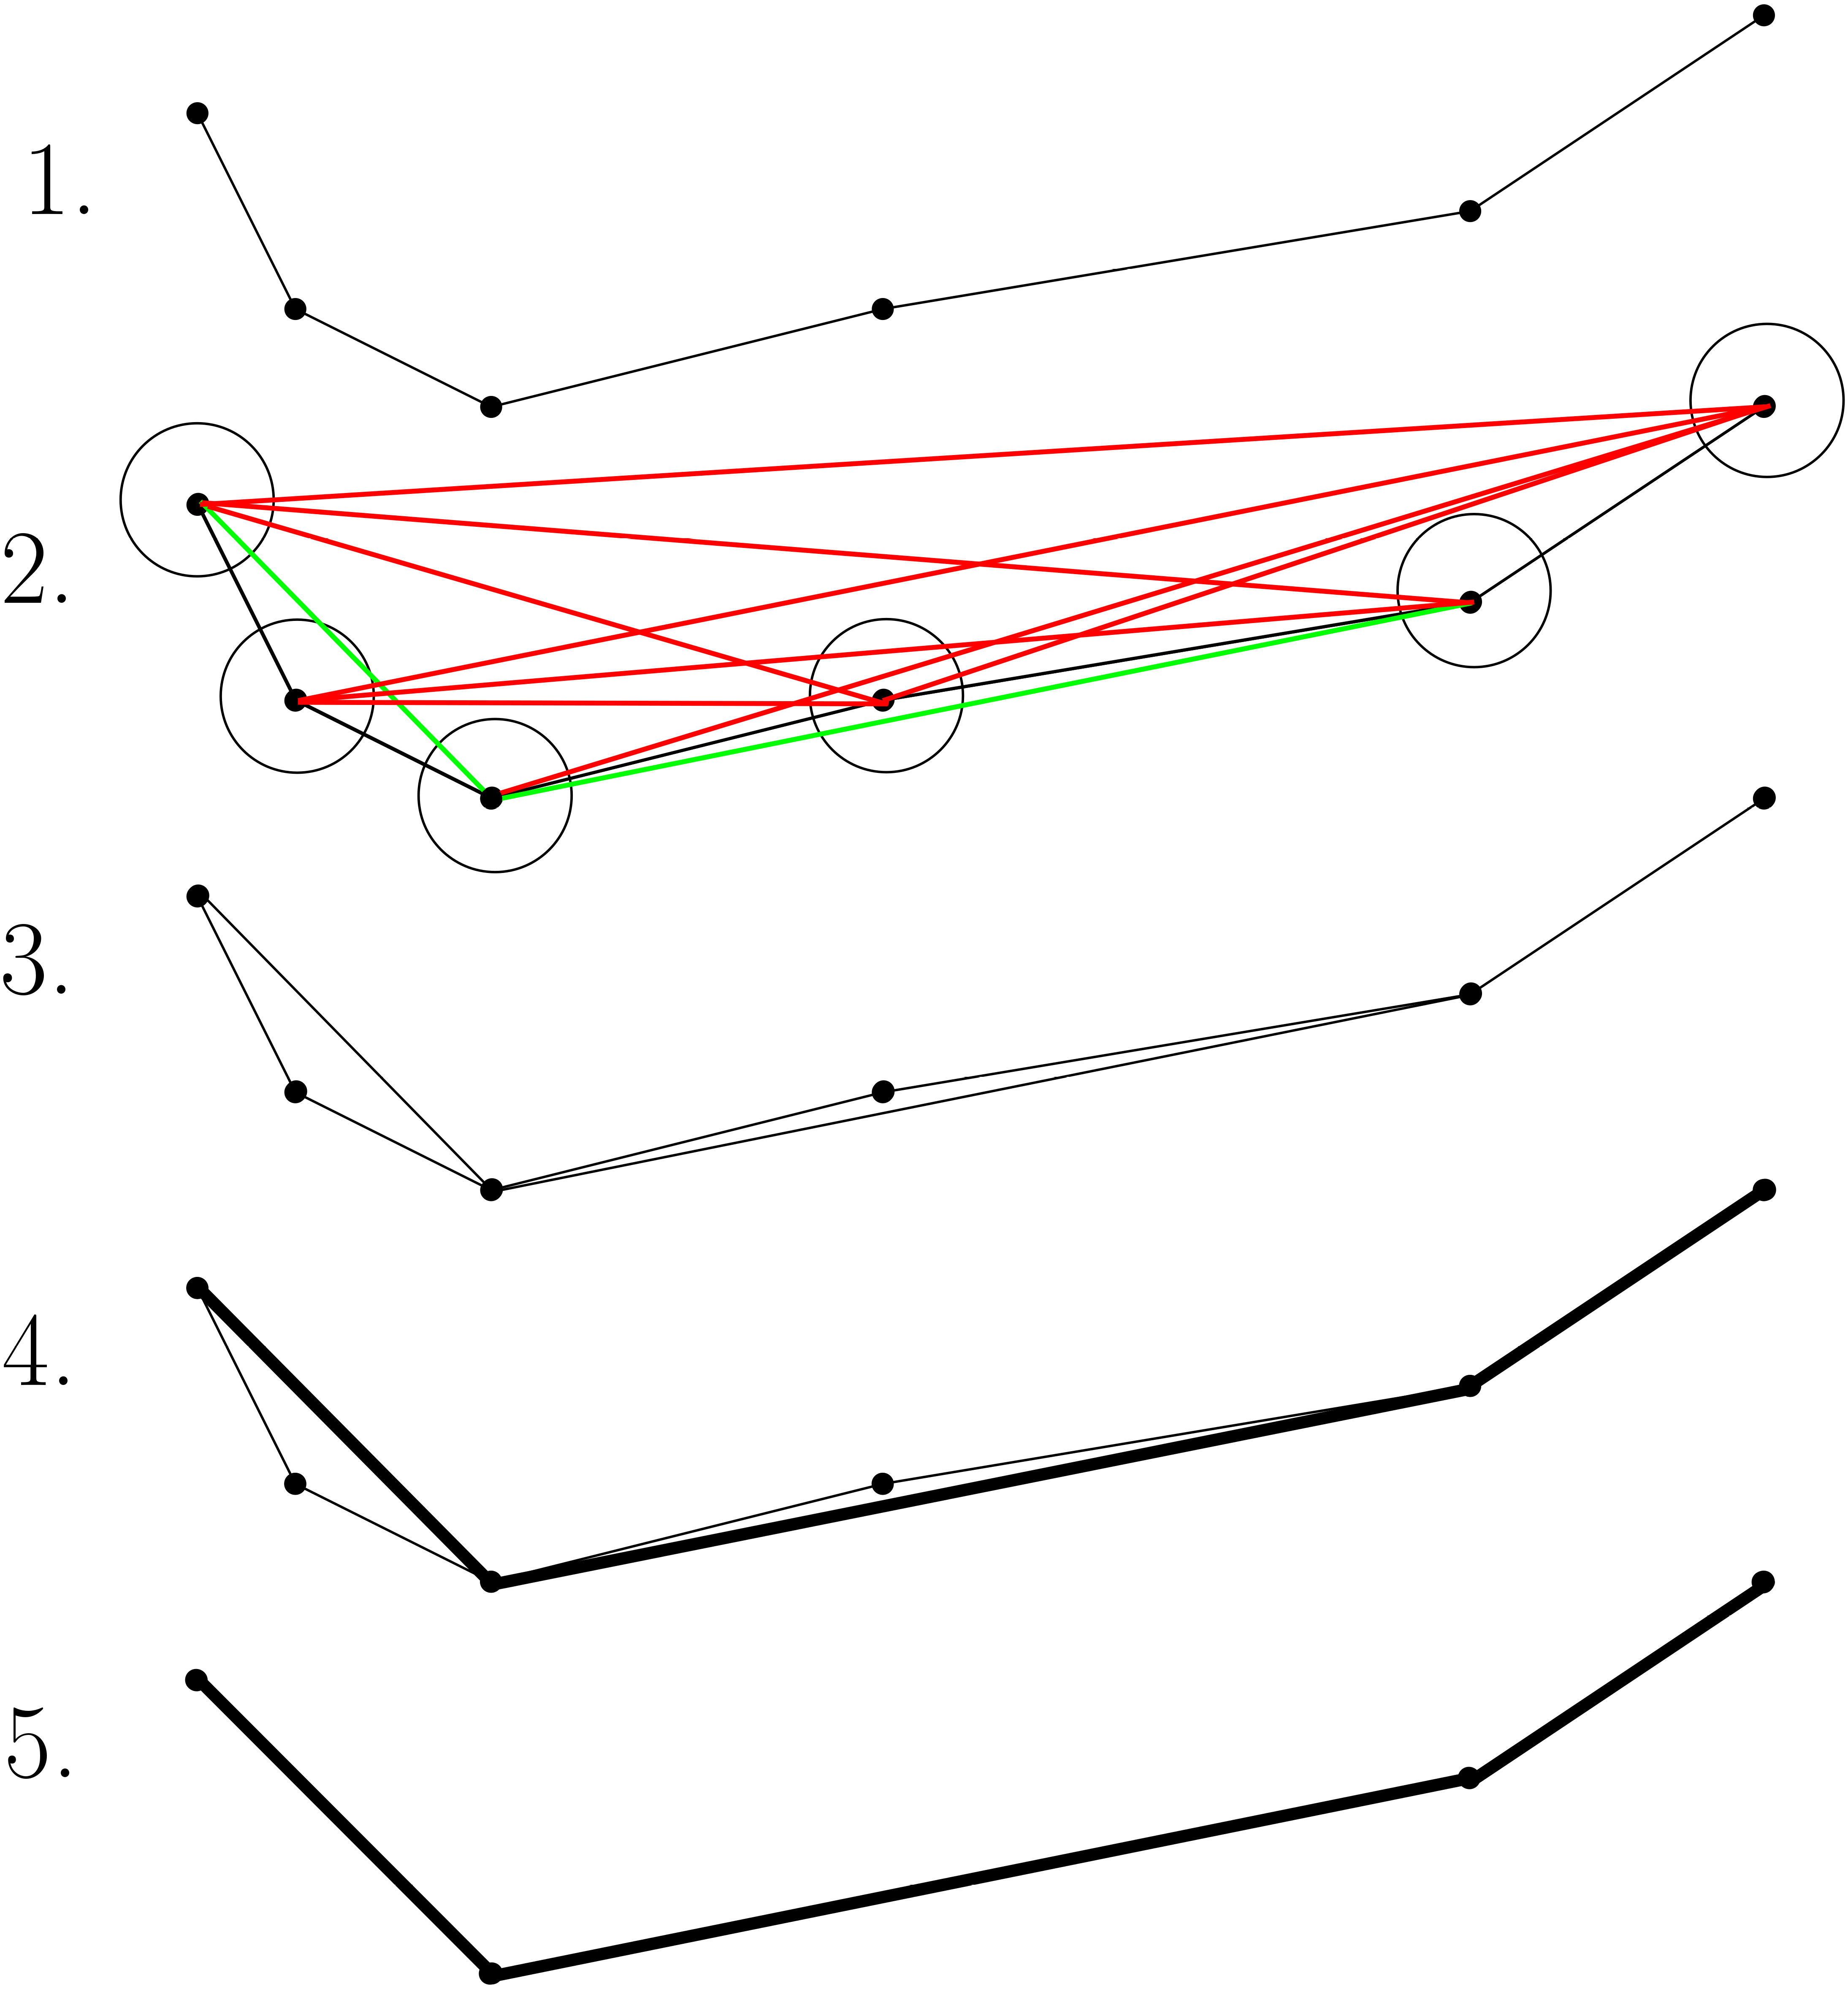
\includegraphics[width=0.5\linewidth]{figures/imaiiri.png}
    \caption{Illustration of how the Imai-Iri algorithm generates
    shortcuts. Green lines are allowed shortcuts, red
    lines are not allowed \cite{van2017extensive}.}
    \label{fig:imai}
\end{figure}

\newpage

\section{Streaming Process Algorithm}

Traditional data-management systems software is built on the concept of persistent
data sets that are stored reliably in stable storage and queried/updated several
times throughout their lifetime. For several emerging application domains, however,
data arrives and needs to be processed on a continuous (24×7) basis, without
the benefit of several passes over a static, persistent data image \cite{garofalakis2016data}.

It is therefore important to have algorithm to process those stream data.

\subsection{Data-Stream}

Perhaps the most basic synopsis of a data stream is a sample of elements from the
stream. A key benefit of such a sample is its flexibility: the sample can serve as input
to a wide variety of analytical procedures and can be reduced further to provide
many additional data synopses \cite{garofalakis2016data}. If, in particular, the sample is collected using random
sampling techniques, then the sample can form a basis for statistical inference
about the contents of the stream. Data-stream sampling problems require the application of many ideas and techniques
from traditional database sampling, but also need significant new innovations,
especially to handle queries over infinite-length streams. Indeed, the unbounded
nature of streaming data represents a major departure from the traditional
setting. We draw an important distinction
between a stationary window, whose endpoints are specified times or specified
positions in the stream sequence, and a sliding window whose endpoints move forward
as time progresses. Examples of the latter type of window include “the most
recent n elements in the stream” and “elements that have arrived within the past
hour.” Sampling from a finite stream is a special case of sampling from a stationary
window in which the window boundaries correspond to the first and last stream
elements. When dealing with a stationary window, many traditional tools and techniques
for database sampling can be directly brought to bear. In general, sampling
from a sliding window is a much harder problem than sampling from a stationary
window: in the former case, elements must be removed from the sample as they
expire, and maintaining a sample of adequate size can be difficult.We also consider
“generalized” windows in which the stream consists of a sequence of transactions
that insert and delete items into the window; a sliding window corresponds to the
special case in which items are deleted in the same order that they are inserted.

In the context of this thesis we will investigate the technology of POSTGIS on data stream and adapt the algorithm based on the techniques used by POSTGIS for data stream.

\subsection{Stream Processing}

Data streams can be generated in various scenarios,
including a network of sensor nodes, a stock market or a
network monitoring system and so on \cite{namiot2015big}. It exist multiple techniques that could be done on
a data stream such as continuous queries,clustering,classification,frequent items mining,outlier and anomaly detection.A stream processing solution has to solve different
challenges \cite{Wähner_2014} :
\begin{itemize}
    \item  Processing massive amounts of streaming events (filter, aggregate, rule, automate, predict, act, monitor, alert)
    \item  Real-time responsiveness to changing market conditions
    \item  Performance and scalability as data volumes increase in size and complexity
    \item  Rapid integration with existing infrastructure and data sources: Input (e.g. market data, user inputs, files, history data from a DWH) and output (e.g. trades, email alerts, dashboards, automated reactions)
    \item  Fast time-to-market for application development and deployment due to quickly changing landscape and requirements
    \item  Developer productivity throughout all stages of the application development lifecycle by offering good tool support and agile development
    \item  Analytics: Live data discovery and monitoring, continuous query processing, automated alerts and reactions
    \item  Community (component / connector exchange, education / discussion, training / certification)
    \item  End-user|ad-hoc continuous query access
    \item  Alerting
    \item  Push-based visualization
\end{itemize}

\subsection{Technologies}
In this section, we discuss some technological solutions for
data streams processing.
Apache Storm is a distributed real-time computation system
for processing large volumes of high-velocity data \cite{jain2014learning}. Is a
distributed real-time computation system for processing fast,
large streams of data. Storm is an architecture based on
master-workers paradigm. So a Storm cluster mainly
consists of a master and worker nodes, with coordination
done by Zookeeper.

Spark Streaming \cite{spark} is an extension of the core Spark API
\cite{shoro2015big} that enables scalable, high-throughput, fault-tolerant
stream processing of live data streams. Data can be ingested
from many sources like Kafka, Flume, Twitter, ZeroMQ,
Kinesis, or TCP sockets, and can be processed using
complex algorithms expressed with high-level functions like
map, reduce, join and window, see Figure \ref{fig:streams}.

\begin{figure}[!h]
    \centering
    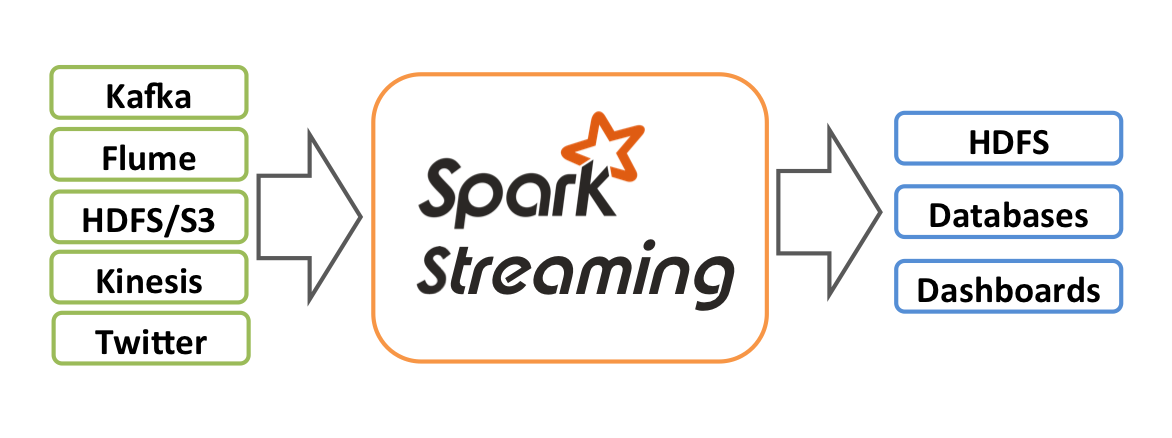
\includegraphics[width=1\linewidth]{figures/streaming-arch.png}
    \caption{Spark Streaming model representation as we can see it can receive multiple data sources and output to multiple data sources \cite{spark}.}
    \label{fig:streams}
\end{figure}



Finally, processed data can be pushed out to files systems,
databases, and live dashboards. In fact, you can apply
Spark’s machine learning and graph processing algorithms
on data streams, see Figure \ref{fig:procs}).

\begin{figure}[!h]
    \centering
    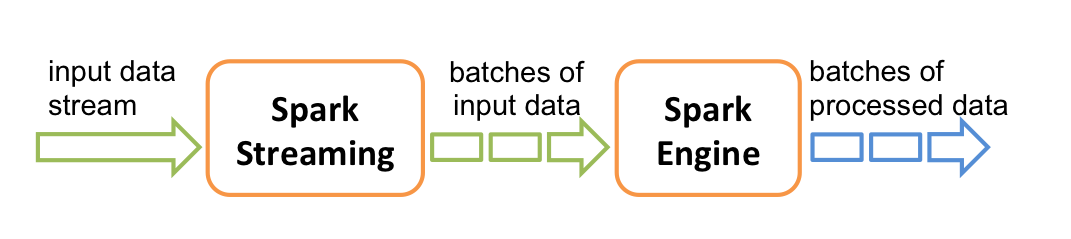
\includegraphics[width=1\linewidth]{figures/streaming-flow.png}
    \caption{Spark Processing \cite{spark}.}
    \label{fig:procs}
\end{figure}



Apache Samza \cite{samza} is a distributed stream processing
framework. It uses Apache Kafka for messaging, and
Apache Hadoop YARN to provide fault tolerance, processor
isolation, security, and resource management see Figure \ref{fig:samza}.

\begin{figure}[!h]
    \centering
    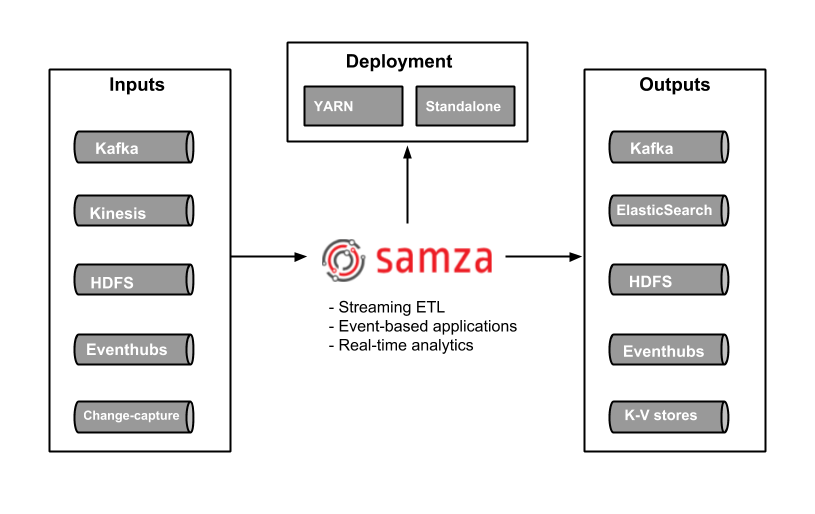
\includegraphics[width=1\linewidth]{figures/samza-arch4.png}
    \caption{Apache Samza \cite{samza}.}
    \label{fig:samza}
\end{figure}



Apache Flume \cite{flume} is a distributed, reliable, and available
service for efficiently collecting, aggregating, and moving
large amounts of log data. It has a simple and flexible
architecture based on streaming data flows. It is robust and
fault tolerant with tunable reliability mechanisms and many
failovers and recovery mechanisms. It uses a simple
extensible data model that supports online analytic
applications see Figure \ref{fig:flume}.

\begin{figure}[!h]
    \centering
    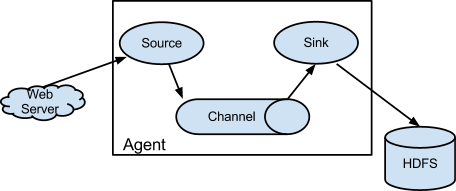
\includegraphics[width=1\linewidth]{figures/DevGuide_image00.png}
    \caption{Apache Flume \cite{flume}.}
    \label{fig:flume}
\end{figure}


Apache Kafka itself is often used as a kernel for data stream
architecture. Originally, Apache Kafka is publish-subscribe
messaging rethought as a distributed commit log \cite{ApacheKA}.
Apache Kafka is a distributed system designed for streams.
It is built to be fault-tolerant, high-throughput, horizontally
scalable, and allows geographically distributing data streams
and processing. See Figure \ref{fig:kafka} illustrates stream-centric
architecture in Confluent blog  \cite{Kafka}.

\begin{figure}[!h]
    \centering
    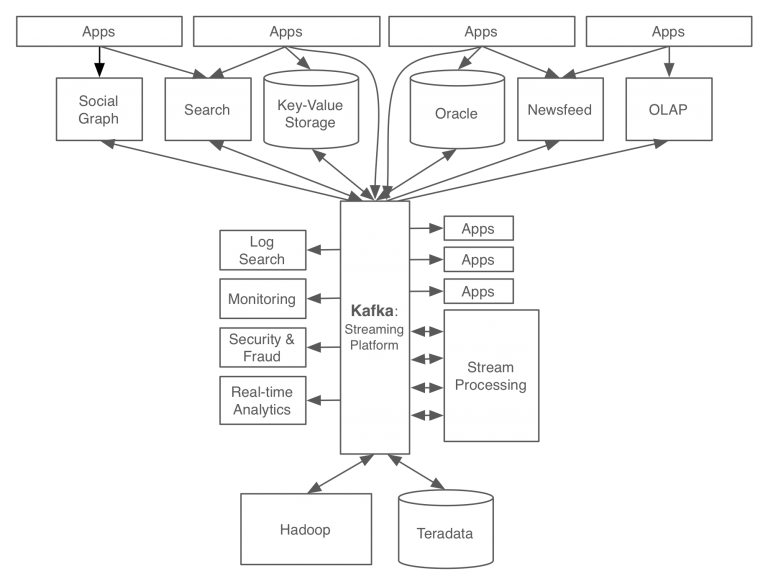
\includegraphics[width=1\linewidth]{figures/data-flow-768x584.png}
    \caption{Stream-centric architecture on Apache Kafka \cite{Kafka}.}
    \label{fig:kafka}
\end{figure}

Amazon Kinesis \cite{kinesis} is a fully managed, cloud-based
service for real-time data processing over large, distributed
data streams. Amazon Kinesis can continuously capture and
store terabytes of data per hour from hundreds of thousands
of sources such as website clickstreams, financial
transactions, social media feeds, IT logs, and locationtracking
events.



IBM InfoSphere Streams \cite{ballard2014ibm,ibmdoc} is an advanced analytic
platform that enables the development and execution
of applications that process information in data streams.
InfoSphere Streams enables continuous and fast analysis of massive volumes
of moving data to help improve the speed of business insight and decision making see Figure \ref{fig:ibm}.

\begin{figure}[!h]
    \centering
    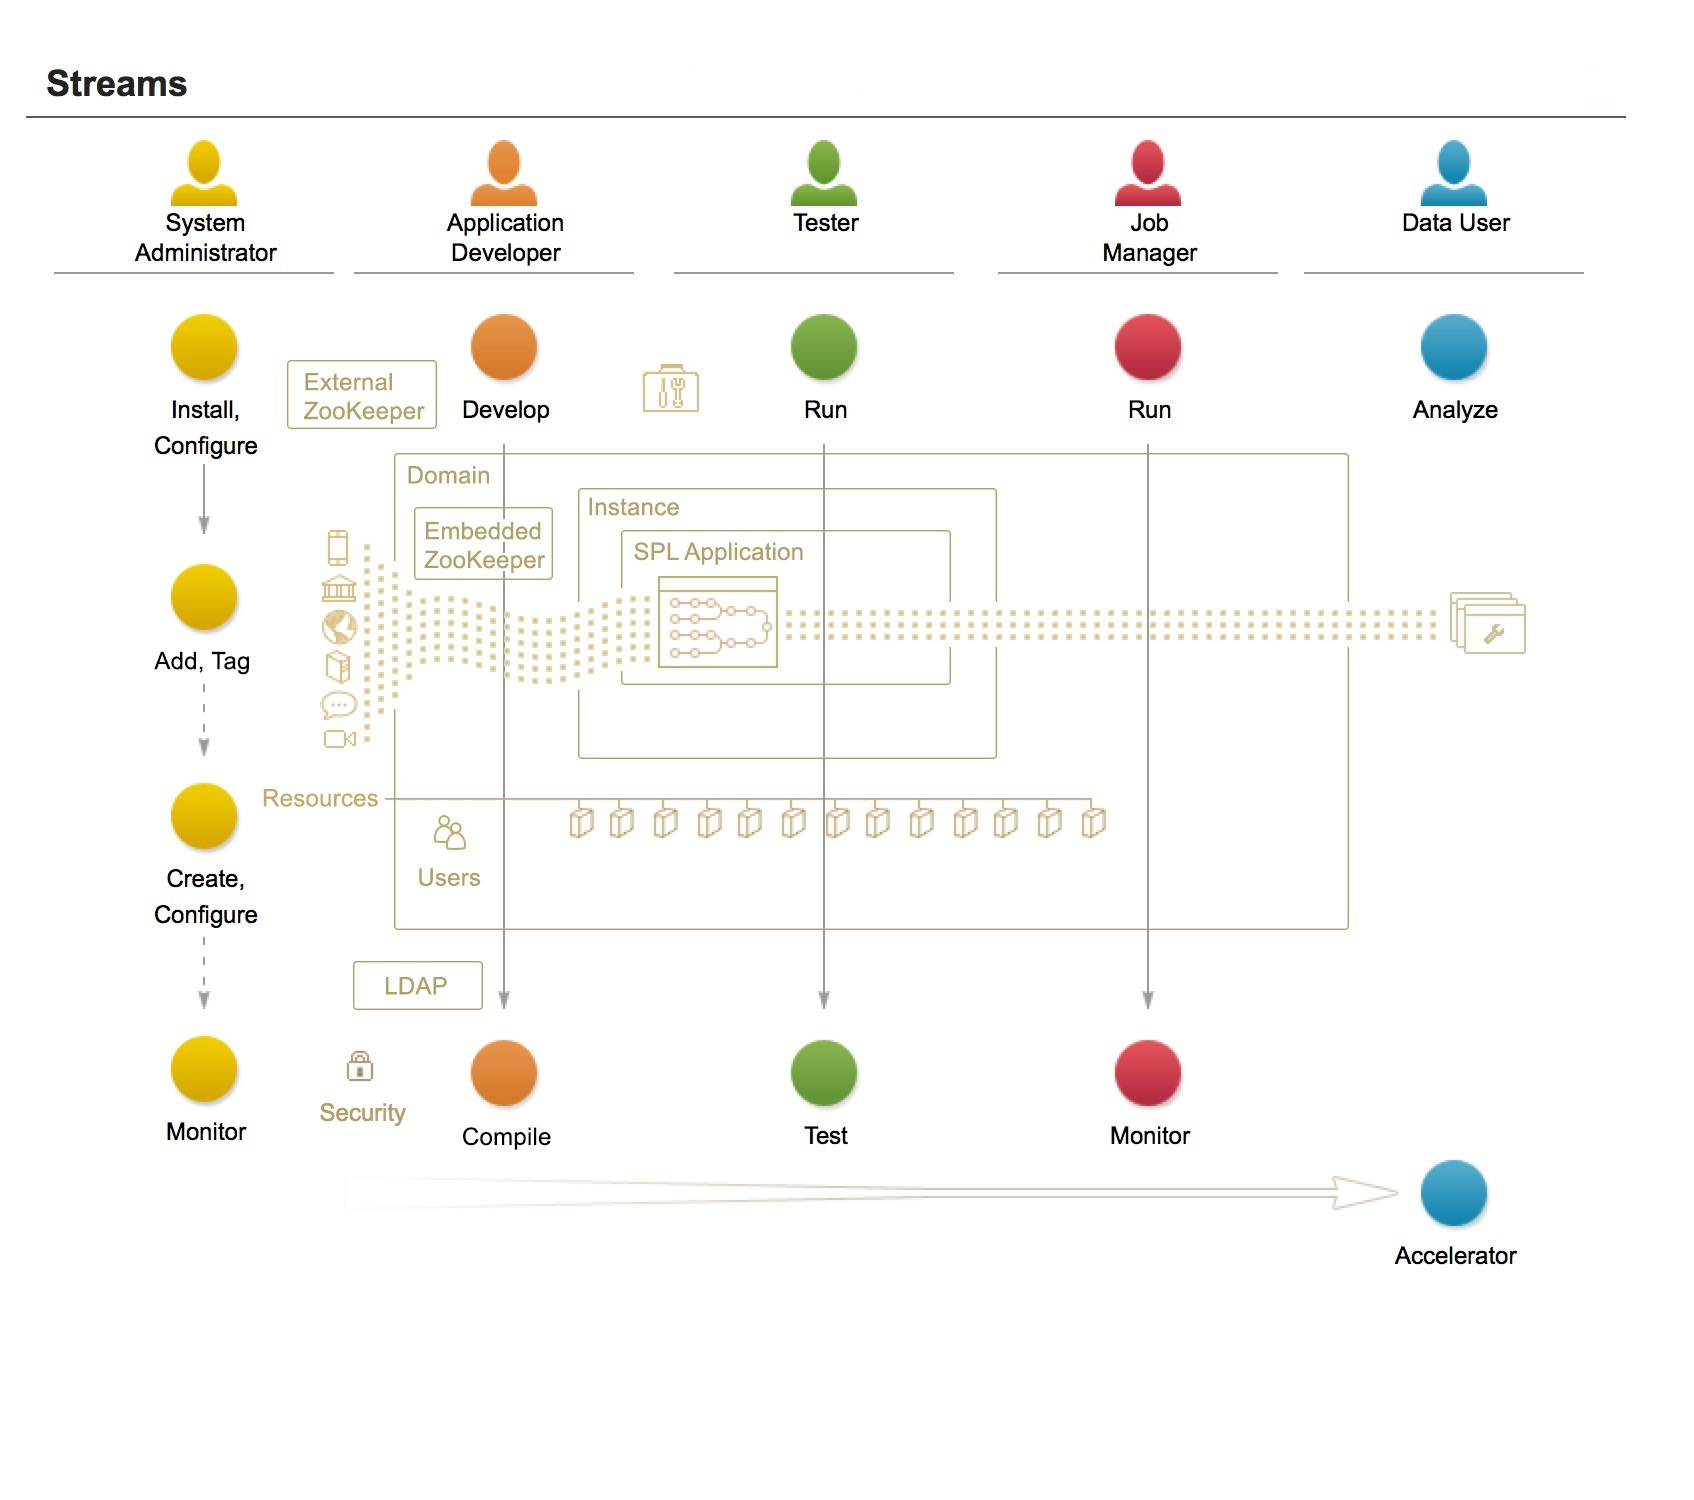
\includegraphics[width=1\linewidth]{figures/model.jpg}
    \caption{IBM InfoSphere Streams \cite{ibmdoc}.}
    \label{fig:ibm}
\end{figure}


\subsection{Streaming for Line Simplification}
In this section we will discuss the current state of line simplification algorithm/problem in the context of stream processing.
The main problematic of this thesis is related to this problem because of that this subject will have a more in depth analysis.

As mentionned in "Streaming algorithms for line simplification" \cite{abam2007streaming}, suppose we are tracking one, or maybe many,
moving objects. Each object is equipped with a device that
is continuously transmitting its position. Thus we are re-
ceiving a stream of data points that describes the path along
which the object moves. The goal is to maintain this path
for each object. We are interested in the scenario where we
are tracking the objects over a very long period of time, as
happens for instance when studying the migratory patterns
of animals. In this situation it may be undesirable or even
impossible to store the complete stream of data points. In-
stead we have to maintain an approximation of the input
path. This leads us to the following problem: we are receiving a (possibly infinite) stream $p0,p1,p2,...$ of points in
the plane, and we wish to maintain a simplification (of the
part of the path seen so far) that is as close to the original
path as possible, while using not more than a given (fixed)
amount of available storage.

\paragraph{Formalization}
In this subsection we will formalize the problem of line simplification in a streaming mode based on the article \cite{abam2007streaming}.
To be able to state the problem we wish to solve and the results we obtain more precisely, we first introduce some terminology and definitions.
Let $p_0, p_1, \ldots$ be the given stream of input points. We use $P(n)$ to denote the path defined by the points
$p_0, p_1, \ldots, p_n$ - that is, the path connecting those points in order - and for any two points $p, q$ on the path we use
$P(p, q)$ to denote the subpath from $p$ to $q$. For two vertices $p_i, p_j$ we use $P(i, j)$ as a shorthand for $P\left(p_i, p_j\right)$.
A segment $p_i p_j$ with $i<j$ is called a link or sometimes a shortcut. Thus $P(n)$ consists of the links $p_{i-1} p_i$ for $0<i \leqslant n$.
We assume a function error is given that assigns a non-negative error to each link $p_i p_j$.
A $\ell$-simplification of $P(n)$ is a polygonal path $Q:=q_0, q_1, \ldots, q_k, q_{k+1}$ where
$k \leqslant \ell$ and $q_0=p_0$ and $q_{k+1}=p_n$, and $q_1, \ldots, q_k$ is a subsequence of
$p_1, \ldots, p_{n-1}$. The error of a simplification $Q$ for a given function error, denoted
$\operatorname{error}(Q)$, is defined as the maximum error of any of its links.

\paragraph{Evaluation}
Now consider an algorithm $\mathcal{A}:=\mathcal{A}(\ell)$ that maintains an $\ell$-simplification for the input stream $p_0, p_1, \ldots$,
for some given $\ell$. Let $Q_{\mathcal{A}}(n)$ denote the simplification that $\mathcal{A}$ produces for the path $P(n)$. Let $\operatorname{Opt}(\ell)$
denote an optimal off-line algorithm that produces an $\ell$-simplification. Thus $\operatorname{error}\left(Q_{O p t(\ell)}(n)\right)$ is the minimum possible
error of any $\ell-$ simplification of $P(n)$. We define the quality of $\mathcal{A}$ using the competitive ratio, as is standard for on-line algorithms.
We also allow resource augmentation. More precisely, we allow $\mathcal{A}$ to use a $2k$-simplification, but we compare the error of this simplification
to $Q_{O p t(k)}(n)$. (This is similar to Agarwal et al. \cite{agarwal2005near} who compare the quality of their solution to the min- $k$ problem for a given maximum error $\delta$
to the optimal value for maximum error $\delta / 2$.) Thus we define the competitive ratio of an algorithm $\mathcal{A}(2 k)$ as
$$
\text { competitive ratio of } \mathcal{A}(2 k):=\max _{n \geqslant 0} \frac{\operatorname{error}\left(Q_{\mathcal{A}(2 k)}(n)\right)}{\operatorname{error}\left(Q_{O p t(k)}(n)\right)},
$$
where $\frac{\operatorname{error}\left(Q_{\mathcal{A}(2 k)}(n)\right)}{\operatorname{error}\left(Q_{O p t(k)}(n)\right)}$ is defined as
1 if $\operatorname{error}\left(Q_{\mathcal{A}(2 k)}(n)\right)=$ $\operatorname{error}\left(Q_{O p t(k)}(n)\right)=0$.
We say that an algorithm is $c$ competitive if its competitive ratio is at most $c$.

\paragraph{Algorithm}
We will discuss the existing algorithm for the line simplification in a streaming model. In the article \cite{abam2007streaming} they propose
the following algorithm. Our algorithm is quite simple. Suppose we have already handled the points $p_0, \ldots, p_n$.
(We assume $n>\ell+1$; until that moment we can simply use all points and have zero error.) Let $Q:=q_0, q_1, \ldots, q_{\ell}, q_{\ell+1}$
be the current simplification. Our algorithm will maintain a priority queue $\mathcal{Q}$ that stores the points $q_i$ with $1 \leqslant i \leqslant \ell$,
where the priority of a point is the error (as computed by the oracle) of the link $q_{i-1} q_{i+1}$. In other words, the priority of $q_i$ is
(an approximation of) the error that is incurred when $q_i$ is removed from the simplification. Now the next point $p_{n+1}$ is handled as follows:

\begin{enumerate}
    \item  Set $q_{\ell+2}:=p_{n+1}$, thus obtaining an $(\ell+1)$-simplification of $P(n+1)$.
    \item  Compute $\operatorname{error}^*\left(q_{\ell} q_{\ell+2}\right)$ and insert $q_{\ell+1}$ into $\mathcal{Q}$ with this error as priority.
    \item  Extract the point $q_s$ with minimum priority from $\mathcal{Q}$; remove $q_s$ from the simplification.
    \item  Update the priorities of $q_{s-1}$ and $q_{s+1}$ in $\mathcal{Q}$.

\end{enumerate}

As we can see the following algorithm is using the error function in order to correct the result in real-time. In the context of this thesis we will investigate a solution
that is based on the existing algorithm douglas-peucker to see if it is possible to maintain a simplified version of the trip using this algorithm.




\subsection{Moving Object Database}
In order to store the position of our tracking objects it is important to
search on moving object database as data output for this thesis. Moving objects are objects that change their value or location
with time. These can be vehicles, persons, animals, aircarft, the air
temperature of a city, the fuel price in a certain gas station, etc.
The ubiquity of tracking devices and IoT technologies has resulted
in collecting massive amounts of data that describe the temporal
evolution of such objects and values. This creates opportunities
to build applications on this data, which in turn calls for building \cite{zimanyi2019mobilitydb}.

As mentioned above the need for a specific database in order to have an efficient data storage.
In the context of this thesis we will focus on mobilityDB which is a Moving Object database that extends
PostgreSQL

\paragraph{PostgreSQL}

PostgreSQL is an object-relational database management system (ORDBMS) based on POSTGRES, Version 4.2,
developed at the University of California at Berkeley Computer Science Department \cite{postgresql}. POSTGRES pioneered many
concepts that only became available in some commercial database systems much later.

PostgreSQL is an open-source descendant of this original Berkeley code. It supports a large part of the SQL standard
and offers many modern features:

\begin{itemize}

    \item complex queries
    \item foreign keys
    \item triggers
    \item updatable views
    \item transactional integrity
    \item multiversion concurrency control
\end{itemize}

Also, PostgreSQL can be extended by the user in many ways, for example by adding new

\begin{itemize}
    \item data types
    \item functions
    \item operators
    \item aggregate functions
    \item index methods
    \item procedural languages
\end{itemize}
And because of the liberal license, PostgreSQL can be used, modified, and distributed by anyone free of charge for any purpose, be it private, commercial, or academic.


\paragraph{PostGIS}
PostGIS represents a potent open-source instrument facilitating the creation of resilient spatial databases. Serving as the geographic extension of the PostgreSQL database management system, PostGIS enables the incorporation of geographic objects within data tables \cite{marquez2015postgis}. These geographic objects are specialized data types designed for the storage of geographic positions or sets thereof, integrated seamlessly into lines or polygons. In essence, PostGIS emerges as a formidable tool, empowering users to manage intricate geographical data proficiently and to visually interrogate such data when employed in conjunction with graphical tools, exemplified by QGIS.

\paragraph{MobilityDB}
MobilityDB uses the abstract data type approach of MOD implementations
\cite{guting2000foundation}. In an extensible relational database system this
amounts to adding user-defined types that can be used as attribute
types inside relations. MobilityDB defines in PostgreSQL and PostGIS
the temporal types: \texttt{tgeompoint}, \texttt{tgeogpoint}, \texttt{tfloat}, \texttt{tint},
\texttt{ttext}, and \texttt{tbool}. These types encode functions from the time
domain to their corresponding base type domains. MobilityDB extends the existential
spatial database by adding a new dimension. It becomes more dynamics and respond to the need
of processing moving object data.



\chapter{Design}
\section{SQUISH-E}
In this section we introduce the SQUISH-E algorithm, present a pseudo-code and analyze its complexity. \\

The SQUISH-E algorithm compresses a trajectory \(T\) by utilizing two parameters, \(\lambda\) and \(\mu\), to strategically minimize the Synchronized Euclidean Distance (SED) error while achieving a specified compression ratio (\(\lambda\)). It operates by compressing \(T\) until further compression would result in an increase in SED error above \(\mu\), with a notable case being SQUISH-E(\(\lambda\)) where setting \(\mu\) to 0 focuses on minimizing SED error to achieve the compression ratio of \(\lambda\). In contrast, SQUISH-E(\(\mu\)) highlights a scenario where \(\lambda\) is set to 1, aiming to maximize the compression ratio without exceeding the SED error threshold defined by \(\mu\). A pivotal aspect of SQUISH-E is its use of a priority queue \(Q\), in which the priority of each point is determined by an upper bound on the SED error that could be introduced by its removal. This mechanism allows SQUISH-E to efficiently identify and remove the point with the lowest priority, i.e., the point whose removal would result in the least increase in SED error, in \(O(\log |Q|)\) time. This process effectively controls the growth of SED error, ensuring the algorithm's efficiency in compressing trajectory data while maintaining the integrity of the spatial information \cite{muckell2014compression}. In order to have a fully online algorithm SQUISH-E(\(\mu\)) is not taken into account and we only take into account SQUISH-E(\(\lambda\)). The error function is the same but in our implementation it could be a nice idea to compare different error function to find the best ones for some situation.

\subsection{Algorithm Pseudo-Code}
In this section we will present the pseudo-code of SQUISH-E algorithm used in our work. \\

\begin{algorithm}[H]
    \DontPrintSemicolon
    \KwIn{trajectory $T$, lower bound $\lambda$ on compression ratio as a percentage value}
    \KwOut{trajectory $T'$}
    $\beta \gets 4$ \tcp*{the initial capacity of $Q$ is 4}
    \ForEach{point $P_i \in T$}{
        \If{$ i * lambda \geq \beta$}{
            $\beta \gets \beta + 1$ \tcp*{increase the capacity of $Q$}
        }
        set\_priority($P_i, \infty, Q$) \tcp*{enqueue $P_i$ with the priority of $P_i$ being $\infty$}
        $\pi[P_i] \gets 0$\;
        \If{$i > 1$}{
            $succ[P_{i-1}] \gets P_i$ \tcp*{register $P_i$ as $P_{i-1}$'s closest successor}
            $pred[P_i] \gets P_{i-1}$ \tcp*{register $P_{i-1}$ as $P_i$'s closest predecessor}
            adjust\_priority($P_{i-1}, Q, pred, succ, \pi$) \tcp*{Algorithm 3}
        }
        \If{$|Q| = \beta$}{
            reduce($Q, pred, succ, \pi$) \tcp*{Algorithm 2}
        }
    }
    \Return{trajectory $T'$ comprising the points in $Q$ in the order reflected in the $succ$ map}
    \caption{SQUISH-E($T, \lambda$)}
    \label{alg:squish_e}
\end{algorithm}

In the algorithm \ref{alg:squish_e} we can analyze the time complexity. The algorithm works iteratively, receiving each point one by one, which is convenient for our streaming case. Complexity is therefore at least $O(n * max(O(loop) ))$ .The lambda variable has also been modified. Next, the following adjust priority \ref{alg:adjust_priority} and reduce  \ref{alg:reduce} algorithms are presented.


\begin{algorithm}[H]
    \DontPrintSemicolon

    \KwIn{priority queue $Q$, maps $\text{pred}, \text{succ}$ and $\pi$ (refer to Table 2)}
    $P_j \gets \text{remove\_min}(Q); \quad$ // the lowest priority point is removed from $Q$\;

    $\pi[succ[P_j]] \gets \text{max}(priority(P_j) , \pi[succ[P_j]]); \quad$  // update neighbor priority\;
    $\pi[pred[P_j]] \gets \text{max}(priority(P_j) , \pi[pred[P_j]]); \quad$ // update neighbor priority\;


    $succ[\text{pred}[P_j]] \gets succ[P_j]; \quad$ // update neighbor's neighbor of $P_j$ \;
    $\text{pred}[succ[P_j]] \gets \text{pred}[P_j]; \quad$ // update neighbor's neighbor of $P_j$ \;


    $\text{adjust\_priority}(\text{pred}[P_j], \text{pred}, \text{succ}, \pi); \quad$ // Algorithm 3\;
    $\text{adjust\_priority}(succ[P_j], \text{pred}, \text{succ}, \pi); \quad$ // Algorithm 3\;
    remove the entry for $P_j$ from $\text{pred}, \text{succ},$ and $\pi; \quad$ // garbage collection\;

    \caption{reduce($Q, \text{pred}, \text{succ}, \pi$)}
    \label{alg:reduce}
\end{algorithm}



\begin{algorithm}[H]
    \DontPrintSemicolon

    \KwIn{point $P_j$, priority queue $Q$, maps $\text{pred}, \text{succ}$ and $\pi$ (refer to Table 2)}
    \If{$\text{pred}[P_j] \neq \text{null}$ and $\text{succ}[P_j] \neq \text{null}$}{
        $p \gets \pi[\text{SED}(P_j,\text{pred}[P_j], \text{succ}[P_j])];$\;
        $\text{set\_priority}(P_j, p, Q);$\;
    }

    \caption{adjust\_priority($P_j, Q, \text{pred}, \text{succ}, \pi$)}
    \label{alg:adjust_priority}
\end{algorithm}


To achieve the optimum complexity of this algorithm, it is imperative that the most expensive operation in the loop is $O(log(n))$. Next, the focus will be on variables and their methods, in order to determine the required implementation elements.

\subsection{Variables}


\begin{table}[h!]
    \centering
    \label{tab:variables}
    \begin{tabular}{ll}
        \hline
        \textbf{Variable} & \textbf{Description} \\
        \hline
        $Q$             & Priority queue \\
        $p_{\pi}$       & Point with the lowest priority \\
        $\text{pred}$   & Predecessor map \\
        $\text{succ}$   & Successor map \\
        $\pi$           & Priority map \\
        $P_i$           & A point in the priority queue \\
        $\text{SED}$    & Some distance function \\
        \hline
    \end{tabular}
    \caption{List of Variables Used in Algorithms}
\end{table}

\paragraph{Map}

As mentioned before we have 3 map two that has as pair key-value point-point and another with point-priority .


\subparagraph{Method}
The method that is necessary to implement for this map is the following

\begin{itemize}
    \item set(key,value,map)
    \item remove(key,map)
    \item get(key,map) -> value
\end{itemize}


\paragraph{PriorityQueue}
Another structure is a priority queue, but with quite different methods.
The priority queue stores elements that are point-priority pairs, and has a sorted structure so that the minimum can be removed. This structure poses a real challenge, due to its nature and the methods we'll define below.


\subparagraph{Method}
The methods required to implement priorityqueue are as follows:
\begin{itemize}
    \item set\_priority(key,value,Q) this function can be expressed as the two following methods
    \begin{itemize}
        \item remove(key,Q) or replace(key,Q) // depends on implementation
        \item push(key,value,Q)
    \end{itemize}
    \item remove\_min(Q)
\end{itemize}

As the set function is closer to the characteristics of an array than a priorityqueue, this poses a challenge if existing resources don't allow these methods to be implemented in $O(log(n))$ at most.






\section{SQUISH-E Implementation}
The following sections focuses on the implementation of the elements described in the previous sections. In order to implement the algorithm, C was chosen because it allows the use of streaming technologies such as Kafka. It also allows the executable to be run at high speed because C is a compiled language, which reduces latency compared with other languages such as Python, which is an interpreted language, and Java, which runs on a Java Virtual Machine (JVM). The second advantage of this implementation choice is the use of the C language in database systems such as PostgreSQL in order to be able to implement the algorithm in MobilityDB.

In order to implement the SQUISH-E algorithm, it is necessary to follow the pseudo code and implement each component, as well as making certain implementation choices for elements that are not present in the C language. First SQUISH-E is a state-based algorithm. It does not return any output and have instead a state and update the state for each input. The output strategy chosen is like the sliding window where the last point are keep and the points are pushed into the database. 

\subsection{Algorithm 1 - SQUISH-E}

The first main loop is written as C function. The function have no return and changes the states of the variables.  This function take all the variables mentionned above it has some types and struct that will be described down. 

\begin{lstlisting}[float=h,language=C, % Spécifie le langage du code
caption={SQUISH-E}, % Légende du listing
label=lst:squish_c, % Étiquette pour référencer le listing
numbers=left,
numberstyle=\tiny\color{gray},
stepnumber=1,
frame=single,
breaklines=true,
postbreak=\mbox{\textcolor{red}{$\hookrightarrow$}\space},
showstringspaces=false
]

void
iteration_simplification_sqe(void *p_i , void *p_j ,
size_t *beta,const double lambda,int i,
Dict *succ,Dict *pred,
PDict  *p,struct PriorityQueue *Q,
bool syncdist,interpType interp ,bool hasz ,uint32_t minpts)
{
	if( i * lambda >= *beta)
	{
		*beta += 1;
	}
	set_priority_queue(p_i,INF,Q);
	set_priority_dict(p_i,0,p);
	if(i >= 1)
	{
		set_point_dict(p_i,p_j,pred);
		set_point_dict(p_j,p_i,succ);
		adjust_priority(p_j,Q,pred,succ,p, syncdist, interp , hasz );
	}
	size_t size = size_queue(Q);
	if(size - *beta == 0 ){
		reduce(Q,pred,succ,p,syncdist, interp , hasz );
	}
}
\end{lstlisting}


This algorithm \ref{lst:squish_c} follow the pseudo code of SQUISH-E it called the set function of the priority queue and the set function of the point map and priority map that will be describe in the section about implementation of variable. Then the reduce function and adjust priority is called in order to reduce if the size meet the treshold and the adjustment for each point that has a predecessor and a successor in order to know the error that it will produce by removing the corresponding point.

\subsection{Algorithm 2 - Reduce}
Then we have the main block of SQUISH-E which is the reduce part.

\begin{lstlisting}[language=C, % Spécifie le langage du code
caption={reduce}, % Légende du listing
label=lst:reduce_c, % Étiquette pour référencer le listing
numbers=left,
numberstyle=\tiny\color{gray},
stepnumber=1,
frame=single,
breaklines=true,
postbreak=\mbox{\textcolor{red}{$\hookrightarrow$}\space},
showstringspaces=false,
float,
floatplacement=H
]

void
reduce(struct PriorityQueue *Q,Dict *pred,Dict *succ,PDict  *p,
bool syncdist,interpType interp ,bool hasz )
{
	struct PriorityQueueElem *entry = remove_min(Q);
	size_t size_before = size_queue(Q);
	
	void * p_j = entry->point;
	double priority = entry->priority;
	
	void * p_i = get_point_dict(p_j,pred);
	void * p_k = get_point_dict(p_j,succ);
	
	double pr_i = get_priority_dict(p_i,p); if(priority > pr_i){ pr_i = priority; }
	double pr_k = get_priority_dict(p_k,p); if(priority > pr_k){ pr_k = priority; }
	
	set_priority_dict(p_k, pr_k ,p);
	set_priority_dict(p_i, pr_i ,p);
	
	set_point_dict(p_i,p_k,succ);
	set_point_dict(p_k,p_i,pred);
	set_point_dict(p_k,p_i,pred);
	
	adjust_priority(p_k ,Q,pred,succ,p,syncdist, interp ,hasz );
	adjust_priority(p_i ,Q,pred,succ,p,syncdist, interp ,hasz );
	
	
	//Delete pointer
	free(entry);
	destroy_elem_PriorityDict(p_j,p);
	destroy_elem_PointDict(p_j,succ);
	destroy_elem_PointDict(p_j,pred);
}

\end{lstlisting}

This algorithm \ref{lst:reduce_c} describe the reduction method as mentioned above remove the lowest priority points from the queue and it update the neighbors. Because we use C langage we free memory of the useless data. Each call is represented by a function in order to simplify implementation and reduce it to pieces of code to be written for each particular variable. This choice of implementation also makes it possible to change the structure. 

\subsection{Algorithm 3 - Adjust Priority} 

\begin{lstlisting}[language=C, % Spécifie le langage du code
caption={adjust\_priority}, % Légende du listing
label=lst:adjust_c, % Étiquette pour référencer le listing
numbers=left,
numberstyle=\tiny\color{gray},
stepnumber=1,
frame=single,
breaklines=true,
postbreak=\mbox{\textcolor{red}{$\hookrightarrow$}\space},
showstringspaces=false,
float,
floatplacement=H
]

void
adjust_priority(void *p_i,struct PriorityQueue *Q, Dict *pred,Dict *succ,PDict  *p,
bool syncdist,interpType interp ,bool hasz )
{

	void * p_h = get_point_dict(p_i,pred);
	void * p_k = get_point_dict(p_i,succ);
	if( p_h != NULL &&  p_k != NULL )
	{
		if(syncdist)
		{
			double priority = get_priority_dict(p_i,p) + SED(p_h,p_i,p_k, interp , hasz );
			set_priority_queue(p_i,priority,Q);
		}
	}
}

\end{lstlisting}
 

This algorithm \ref{lst:adjust_c} is what differentiates SQUISH from SQUISH-E: when a point is removed, the surrounding points are updated and their priority changed, so we only recover the neighbours and calculate the new priority on the basis of the old error present in the dictionary and the calculation of the synchronised Euclidean distance. 


\section{Variables Implementation}
In this section we'll discuss how the variables have been implemented and how effective they are, followed by a discussion of the performance and complexity achieved.

\subsection{Map}
In this section we will focus on the implementation of the map

\begin{lstlisting}[float=h,language=C, % Spécifie le langage du code
caption={Map C implementation}, % Légende du listing
label=lst:map_c, % Étiquette pour référencer le listing
numbers=left,
numberstyle=\tiny\color{gray},
stepnumber=1,
frame=single,
breaklines=true,
postbreak=\mbox{\textcolor{red}{$\hookrightarrow$}\space},
showstringspaces=false
]

#include <search.h>


typedef struct PriorityDict
{
void * key;
double priority;
} PriorityDict;


typedef struct PointDict
{
void *key;
void *value;
} PointDict;


typedef void* Dict;
typedef void* PDict;

\end{lstlisting}
 

This structure \ref{lst:map_c} is a Map that link a point to a corresponding value like priority or another point. We just need to define a struct with two values the key and the value. The typedef void* is using for the GNU Library to avoid using void** and add more clarity to the code.

\paragraph{Method}

\begin{lstlisting}[float=h,language=C, % Spécifie le langage du code
caption={Point Map Methods}, % Légende du listing
label=lst:pmap_c, % Étiquette pour référencer le listing
numbers=left,
numberstyle=\tiny\color{gray},
stepnumber=1,
frame=single,
breaklines=true,
postbreak=\mbox{\textcolor{red}{$\hookrightarrow$}\space},
showstringspaces=false
]

void *
get_point_dict(void *p_i,Dict *dict)
{
	PointDict find;
	find.key = p_i;
	void * result = tfind(&find, dict, compar);
	if(result){
		result = (*(PointDict**)result)->value;
	}
	return result;
}

void
set_point_dict(void * p_i,void * p_j,Dict *dict)
{
	PointDict *find = malloc(sizeof(PointDict));
	find->key = p_i;
	find->value = p_j;
	void * result = tfind(find, dict, compar);
	if(result){
		(*(PointDict**)result)->value = p_j;
	}
	else{
		tsearch(find, dict, compar); /* insert */
	}
}

void destroy_elem_PointDict(void * p_i,Dict *dict)
{
	PointDict find;
	find.key = p_i;
	void * r = tfind(&find, dict, compar);
	if(r)
	{
		PointDict * to_free = (*(PointDict**)r);
		tdelete(&find,dict,compar);
		free(to_free);
	}
}

\end{lstlisting} 

Here \ref{lst:pmap_c} we use function of GNU C Library that implement a binary tree. It has the property to have for each operation a maximal complexity of $O(log(n))$ The two mapping use the same implementation in reality it would be a good idea to resolve this duplication case using a template or thing that can resolve it but the C language limit the capability.

\paragraph{Discussion}
As mentioned in the previous sub section the map use GNU C Library binary tree structure to perform search and set. Those algorithm have a complexity of $O(log(n))$ as mentioned before and it has the property to be have a dynamic allocation of memory.

\subsection{PriorityQueue}

\begin{lstlisting}[float=h,language=C, % Spécifie le langage du code
caption={PriorityQueue}, % Légende du listing
label=lst:prqueue_c, % Étiquette pour référencer le listing
numbers=left,
numberstyle=\tiny\color{gray},
stepnumber=1,
frame=single,
breaklines=true,
postbreak=\mbox{\textcolor{red}{$\hookrightarrow$}\space},
showstringspaces=false
]

typedef struct PriorityQueueElem
{
	void * point;
	double priority;
	int index; //reference his own index
} PriorityQueueElem;

typedef void* IDict;

typedef struct PriorityQueue
{
	PriorityQueueElem **arr;
	IDict dict;
	size_t size;
	size_t capacity;
} PriorityQueue;

\end{lstlisting} 

This structure \ref{lst:prqueue_c} implements the function of a priority queue using the structure of a min heap. It has as value PriorityQueueElem which have the point and the corresponding priority and a reference to this index in the heap. The main structure is using an array of pointer of PriorityQueueElem as long as an index map, a int that represent the number of points in the queue and lastly the numbers points allocated.

\paragraph{Method}

Once the skeleton of the algorithm has been implemented. To finish the implementation, the methods of the variables described can be implemented. 

\begin{lstlisting}[float=h,language=C, % Spécifie le langage du code
	caption={PriorityQueue Remove Min}, % Légende du listing
	label=lst:prqueueMethodR_c, % Étiquette pour référencer le listing
	numbers=left,
	numberstyle=\tiny\color{gray},
	stepnumber=1,
	frame=single,
	breaklines=true,
	postbreak=\mbox{\textcolor{red}{$\hookrightarrow$}\space},
	showstringspaces=false
]
	
PriorityQueueElem *remove_min(PriorityQueue *Q)
{
	PriorityQueueElem *result = NULL;
	if (Q->size != 0) {
		result = Q->arr[0];
		// Replace the deleted node with the last node
		Q->arr[0] = Q->arr[Q->size - 1];
		Q->arr[Q->size - 1] = NULL;
		if(Q->arr[0]){
			Q->arr[0]->index = 0;
		}
		
		// Decrement the size of heap
		Q->size--;
		
		tdelete(result,&Q->dict,compar_index);
		// Call minheapify_top_down for 0th index
		// to maintain the heap property
		minHeapify(Q, 0);
	}
	return result;
}
\end{lstlisting}

So, in order to remove the point with the minimum result, the following procedure \ref{lst:prqueueMethodR_c} is used: we check the number of elements and retrieve the first element. The insertion methods ensure that the first element is always the one with the minimum result. Then we take the last element and remove it and place it at the beginning of the queue and balance the tree to keep the smallest element at index 0. Then remove the index from the dictionary. 


\begin{lstlisting}[float=h,language=C, % Spécifie le langage du code
caption={PriorityQueue Set Elem}, % Légende du listing
label=lst:prqueueMethodSet_c, % Étiquette pour référencer le listing
numbers=left,
numberstyle=\tiny\color{gray},
stepnumber=1,
frame=single,
breaklines=true,
postbreak=\mbox{\textcolor{red}{$\hookrightarrow$}\space},
showstringspaces=false
]

void
set_priority_queue(void *p_i,double priority ,PriorityQueue *Q)
{
	struct PriorityQueueElem * insert = replace_elem(p_i,priority,Q);
	if(insert == NULL){
		insert = malloc(sizeof(struct PriorityQueueElem));
		insert->point = p_i;
		insert->priority = priority;
		insert->index = -1;
		tsearch(insert, &Q->dict, compar_index); /* insert */
	}
	if(insert->index == -1){
		push(insert,Q);
	}
}


struct PriorityQueueElem *
replace_elem(void *p_i,double priority ,PriorityQueue *Q)
{
	PriorityQueueElem *elem = get_elem(p_i,&Q->dict);
	if(elem ){
		if(Q->size > elem->index && elem->index != -1){
			Q->arr[elem->index]->priority = priority;
			insertHelper(Q, elem->index);
			minHeapify(Q, elem->index);
		}
	}
	return elem;
}
	
void
push(PriorityQueueElem * insert,PriorityQueue *Q)
{
	Q->size++;
	if(Q->size > Q->capacity){
		Q->arr = realloc(Q->arr, Q->size * sizeof(PriorityQueueElem*));
	}
	Q->arr[Q->size-1] = insert;
	Q->arr[Q->size-1]->index = Q->size-1;
	insertHelper(Q, Q->size-1);
}

\end{lstlisting}

From other implementation this one \ref{lst:prqueueMethodSet_c} has the property to have at most a complexity of $O(log(n))$ the choice of a min heap to implement the priorityqueue fullfill the complexity limitation that we see in the design phase. The min heap is structure has a structure of a tree like we see in Figure \ref{fig:min_heap} and has the property that each tree and sub tree has the property that the parent nodes is always lesser than the child nodes. The min heap implementation is inspired from this website \cite{GfG_2023}. 


\begin{figure}[!h]
\centering
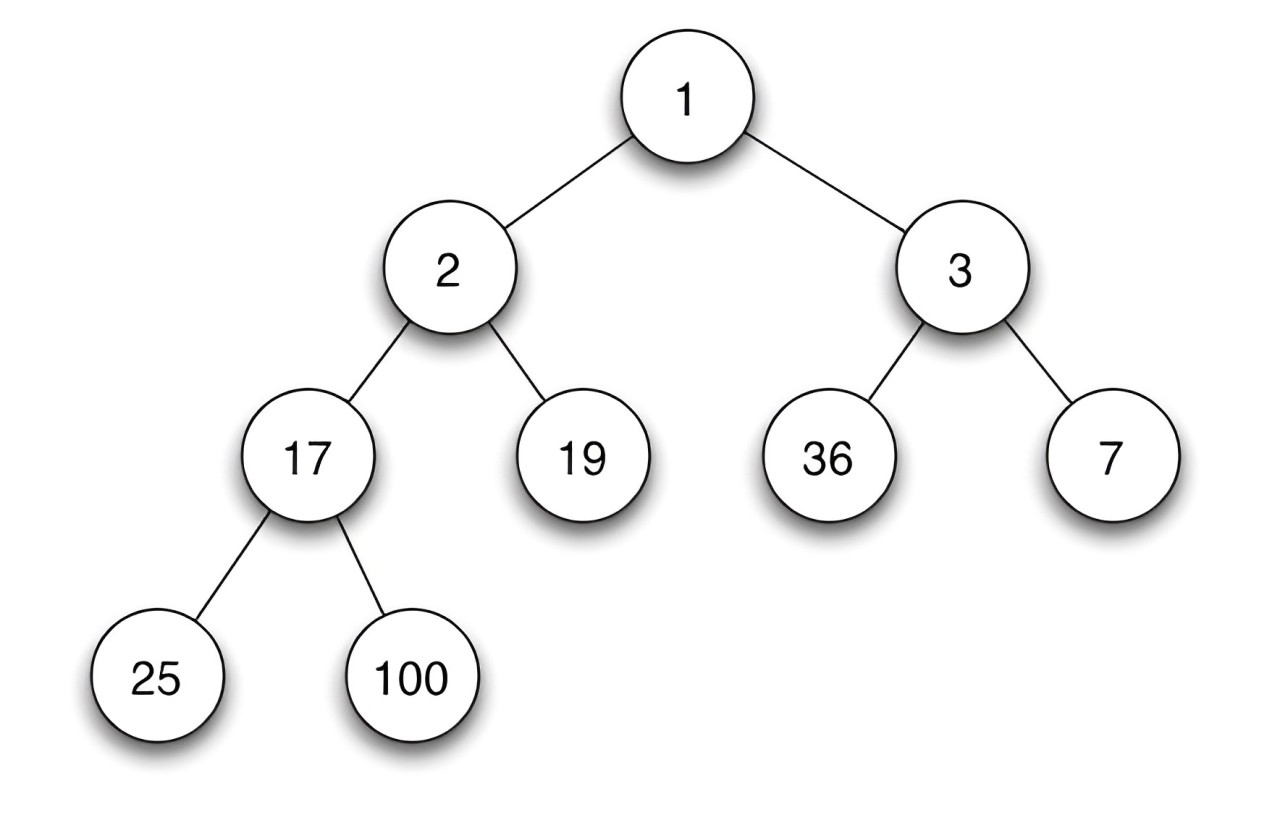
\includegraphics[width=1\linewidth]{figures/tree.jpeg}
\caption{Min Heap Structure}
\label{fig:min_heap}
\end{figure}


\paragraph{Discussion}

The idea here is to use the min heap structure to obtain in a complexity of maximum $O(log(n))$  the point with the lowest priority. In the side we use a index map in order to replace point in the heap in an efficient way. Due to the fact that the design include the set of an element when it is already in the array. This structure has the advantage to benefit from static memory. The set works using the mapping to see if the point is already present in the map. If it is we replace it in the heap by changing his priority and apply a check with his ancestor then his descendant. If the point is not present we add a value at the end of the heap and check and update their ancestor to satisfy the condition of a min heap. So at the end the two operations needed for the algorithm reach a complexity of $O(log(n))$

\section{PostgreSQL Implementation}

In this section we describe how the algorithm is implemented into the MobilityDB sql functions.
\subsection{SQL Code}
As the implementation is in C, the implementation of the sql code \ref{lst:squish_sql} is only a reference to the C function.\\

\begin{minipage}{\linewidth}
\begin{lstlisting}[
language=SQL, % Setting the language for SQL
caption={SQUISHE SQL Code}, % Caption for the listing
label=lst:squish_sql, % Label for referencing the listing
basicstyle=\ttfamily\small, % Basic style
keywordstyle=\color{blue}\ttfamily, % Style for keywords
stringstyle=\color{red}\ttfamily, % Style for strings
commentstyle=\color{green}\ttfamily, % Style for comments
numbers=left, % Line numbers on the left
numberstyle=\tiny\color{gray}, % Style for line numbers
stepnumber=1, % Line numbers step
frame=single,
breaklines=true, % Automatic line breaking
postbreak=\mbox{\textcolor{red}{$\hookrightarrow$}\space}, % Arrow for line breaks
showstringspaces=false % Don't show special spaces within strings
]
CREATE FUNCTION SquishESimplify(tfloat, float, boolean DEFAULT TRUE)
RETURNS tfloat
AS 'MODULE_PATHNAME', 'Temporal_simplify_sqe'
LANGUAGE C IMMUTABLE STRICT PARALLEL SAFE;
CREATE FUNCTION SquishESimplify(tgeompoint, float, boolean DEFAULT TRUE)
RETURNS tgeompoint
AS 'MODULE_PATHNAME', 'Temporal_simplify_sqe'
LANGUAGE C IMMUTABLE STRICT PARALLEL SAFE;
\end{lstlisting}
\end{minipage}

\subsection{Example}
This section show some examples of usages of the pgsql function describe in \ref{lst:squish_sql}. This allowed to use the algorithm in an offline settings using request.\\


\begin{minipage}{\linewidth}
\begin{lstlisting}[
language=SQL, % Setting the language for SQL
caption={Example SQL Code}, % Caption for the listing
label=lst:example_sql, % Label for referencing the listing
basicstyle=\ttfamily\small, % Basic style
keywordstyle=\color{blue}\ttfamily, % Style for keywords
stringstyle=\color{red}\ttfamily, % Style for strings
commentstyle=\color{green}\ttfamily, % Style for comments
numbers=left, % Line numbers on the left
numberstyle=\tiny\color{gray}, % Style for line numbers
stepnumber=1, % Line numbers step
frame=single,
breaklines=true, % Automatic line breaking
postbreak=\mbox{\textcolor{red}{$\hookrightarrow$}\space}, % Arrow for line breaks
showstringspaces=false % Don't show special spaces within strings
]

SELECT SquishESimplify(tfloat '[1@2000-01-01, 2@2000-01-02, 3@2000-01-04,
4@2000-01-05]', '1 day');
-- [1@2000-01-01, 3@2000-01-04]

SELECT asText(SquishESimplify(tgeompoint '[Point(1 1 1)@2000-01-01,
Point(2 2 2)@2000-01-02, Point(3 3 3)@2000-01-04, Point(5 5 5)@2000-01-05)', 0.5));
-- [POINT Z (1 1 1)@2000-01-01, POINT Z (3 3 3)@2000-01-04,POINT Z (5 5 5)@2000-01-05)

\end{lstlisting}
\end{minipage}


\chapter{Experimental Evaluation}

In this chapter it will be discussed the function's effective performance and examine the accuracy and effectiveness of the queries. To compare the offline and online executions, we will also balance the differences between it in real time with the C implementation handling the same data.

\section{Performance}
This section will analyze and discuss the performance of the sql function by varying the lambda parameter and the number of points.
\begin{table}[htbp]
    \centering
    \label{tab:execution_time}
    \begin{tabular}{@{}lccccc@{}}
        \toprule
        Number of Points & \multicolumn{5}{c}{Lambda} \\
        \cmidrule{2-6}
        & 1         & 0.75       & 0.5        & 0.25       & 0.01       \\
        \midrule
        100              & 00.001137 & 00.001965 & 00.002775 & 00.003328 & 00.004529 \\
        1000             & 00.01498  & 00.014966 & 00.022183 & 00.024588 & 00.023035 \\
        10000            & 00.164196 & 00.215692 & 00.214011 & 00.247379 & 00.218447 \\
        100000           & 01.77365  & 02.171435 & 02.844324 & 02.617976 & 02.437037 \\
        1000000          & 04.618455 & 05.371317 & 06.461961 & 06.021071 & 04.510934 \\
        \bottomrule
    \end{tabular}
    \caption{Average Execution Time by Number of Points and Lambda}
\end{table}

In order to get those results we benchmark the request 10 times for each requests and retrieve the average of those executions. As standalone results it has no real meaning outside but we can notice that the speed of the algorithm increase around $0.5$ and decrease outside those values of lambda. We can also state that maybe there is another value as maximum execution time between $0.75$ and $0.25$ . We can state that this is maybe because the number of instruction that mix setting in a priority queue and the instructions of reduction is around $0.5$. Because when lambda is equal to 1 there is no reduction and only setting in the maximal size of a priority queue and adjust priority operation and when lambda go towards $0$ there is a lot of reduction operation and setting in the minimal size of a priority queue. That is an explanation that could befit those data. When the size of the input is multiplying by $10$ the execution time is around $2$ times longer.

\subsection{Comparison with C}
In order to have meaning to those result we will compare it with the C implementation using the real time approach and to see between the offline and the online approach the difference that happen.

\begin{table}[htbp]
    \centering
    \label{tab:execution_time_c}
    \begin{tabular}{@{}lccccc@{}}
        \toprule
        Number of Points & \multicolumn{5}{c}{Lambda} \\
        \cmidrule{2-6}
        & 1         & 0.75       & 0.5        & 0.25       & 0.01       \\
        \midrule
        100              & 00.000094 & 00.000092 & 00.00009 & 00.000098 & 00.000096 \\
        1000             & 00.00081  & 00.000822 & 00.000943 & 00.000876 & 00.000788 \\
        10000            & 00.008889 & 00.008852 & 00.008663 & 00.008263 & 00.00818 \\
        100000           & 00.090018  & 00.088485 & 00.089533 & 00.089064 & 00.088728 \\
        1000000          & 00.892172 & 00.864116 & 00.870661 & 00.937186 & 00.920517 \\
        \bottomrule
    \end{tabular}
    \caption{Average Execution Time (C) by Number of Points and Lambda}
\end{table}

As we can see, executing C code is much faster than executing sql queries, which makes execution and simplification using steam processing techniques in C both viable and possible. The speed is such that even for 1 million points the average execution time is less than 1 second.

\section{Precision}
This section will focus on the precision of the simplification using the same parameter as before in order to have an idea of the quality of the simplification in a function of lambda and types of path. We will discuss on trajectory based on AIS dataset. As stated in \cite{abam2007streaming}, there is different type of path as convex and concave. As a reminder this work focus on the simplification of lines and do not take into account land or see restriction during the simplification process. In this section we will analyze different trajectory defines them and see with different lambda and metrics evaluation the quality of the simplification. At the end we will run in a big datasets and see the results as a graph and discuss them.

\subsection{Trajectory 1}

\begin{figure}[!h]
    \centering
    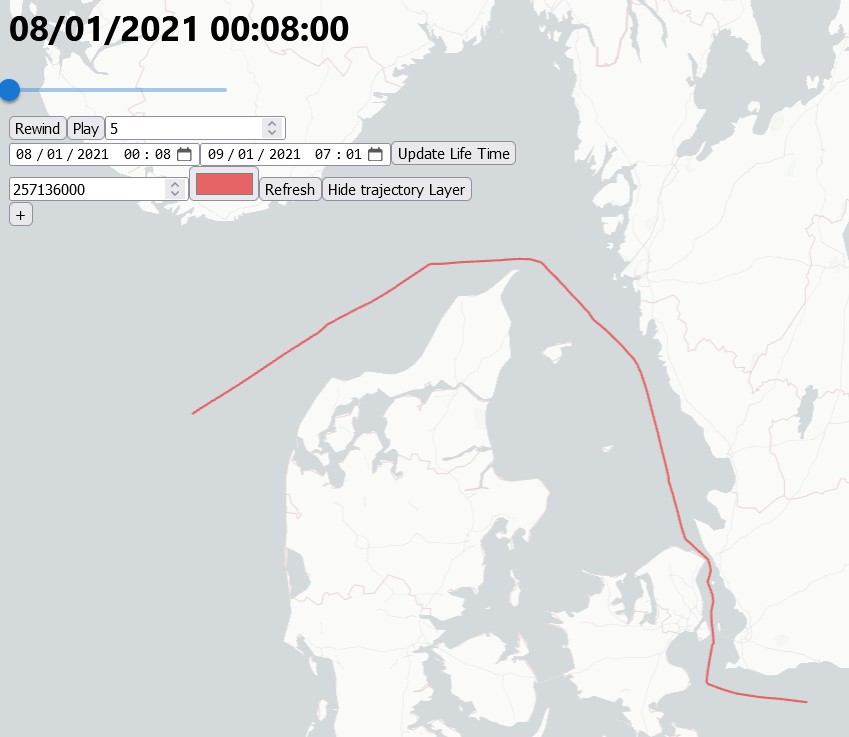
\includegraphics[width=0.5\linewidth]{figures/Stats/traj_1.jpg}
    \caption{Trajectory 1}
    \label{fig:traj_1}
\end{figure}

This trajectory is composed of 20865 points and begin at 1am the 8/1/2021 with a duration of 1 day. This trajectory have convex and concave path in order to analyze the effect of the simplification in those specific moment. The precision of the trajectory will be computed based on the current metrics proposed in the state of the art such as Frechet distance and Hausdorff distances. We will not discuss the precision of lambda 1 because it does not reduce any points from the original trajectory.



\begin{figure}[!h]
    \centering
    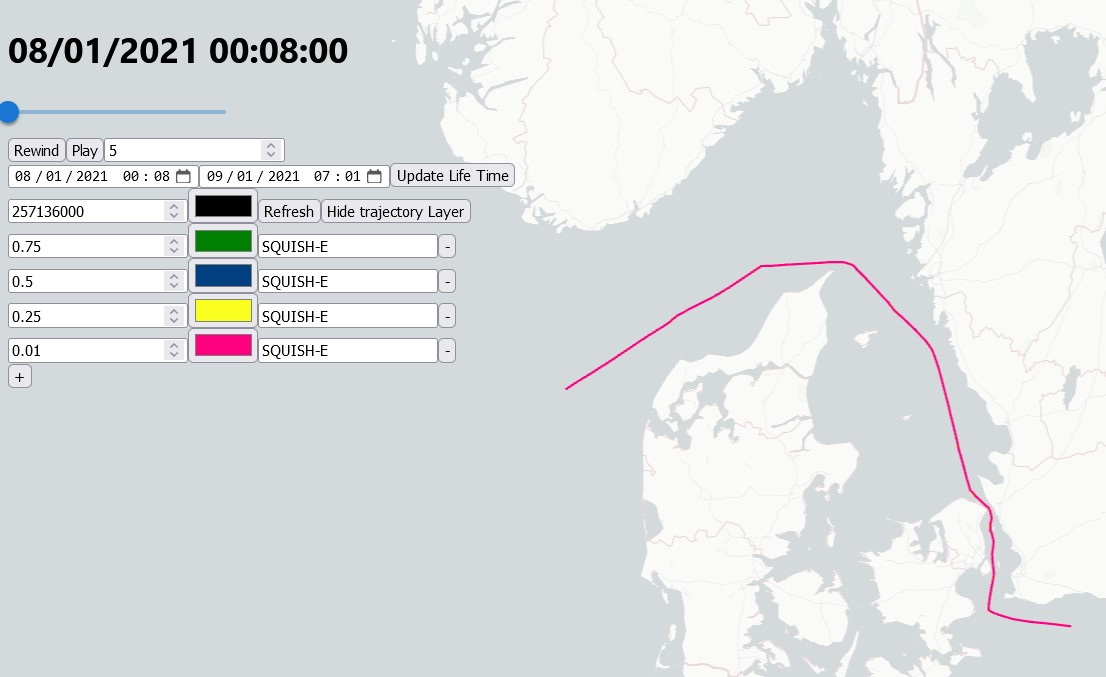
\includegraphics[width=0.5\linewidth]{figures/Stats/squish_1.jpg}
    \caption{Trajectory 1 - SQUISH-E}
    \label{fig:traj_1_squish}
\end{figure}

The path looks really similar and is close to the original path in \ref{fig:traj_1_squish}. In order to see the differences we can zoom and move the slider in order to see the moving objects in relation with the current time.

\begin{figure}[!h]
    \centering
    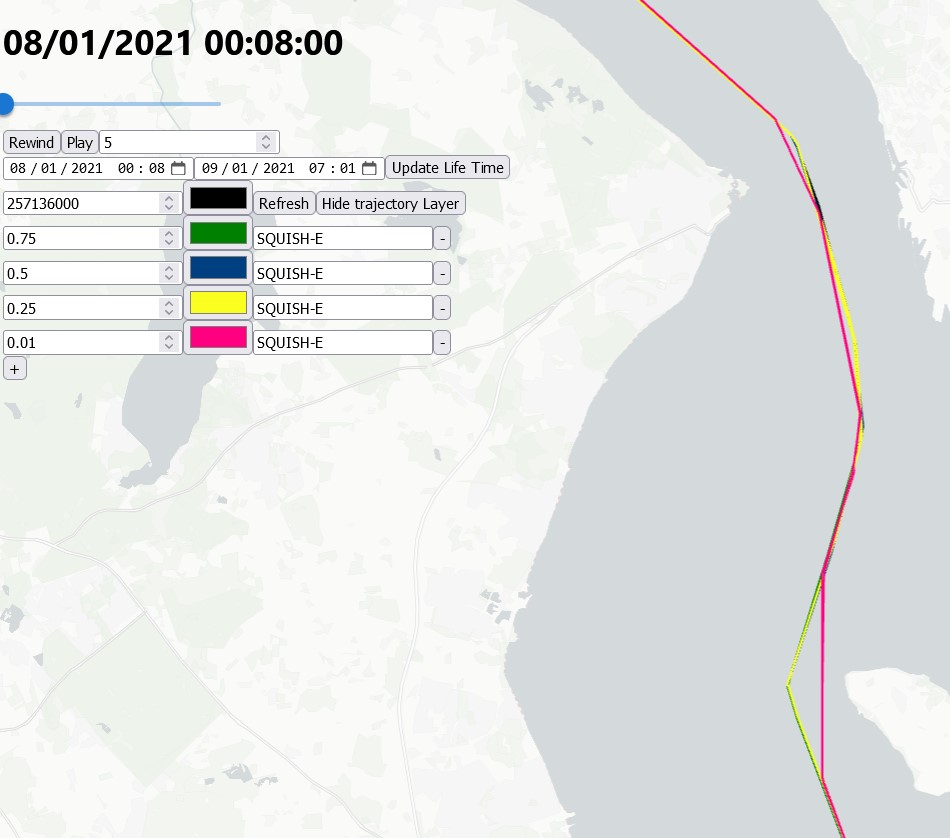
\includegraphics[width=0.5\linewidth]{figures/Stats/squish_1_zoom.jpg}
    \caption{Trajectory 1 - ZOOM }
    \label{fig:traj_1_sqzoom}
\end{figure}

In this we can see the path being simplified where there is curves and having less precision as lambda decreases.

\begin{table}[htbp]
    \centering
    \label{tab:precision_metrics}
    \begin{tabular}{@{}lcccc@{}}
        \toprule
        & \multicolumn{4}{c}{Lambda} \\
        \cmidrule{2-5}
        & 0.75       & 0.5        & 0.25       & 0.01       \\
        \midrule
        Number of points           & 15648 & 10432 & 5215 & 208 \\
        Frechet Distance              & 818.006 & 818.006 & 818.006 & 6902.445 \\
        Hausdorff Distance             & 818.006 & 818.006 & 818.006 & 6902.445 \\
        DynTimeWarp Distance            & 80452.262 &  236389.238 & 634626.475 & 22557588.744\\
        Temporal Distance            & 0.909 & 1.712 & 2.635 & 49.748\\
        \bottomrule
    \end{tabular}
    \caption{Precision metrics per Lambda for Trajectory 1 }
\end{table}

This table gives a view of the precision of SQUISH-E on the first trajectory. The data shows that it is consistent and precise and that errors is increasing when lambda decreases. Dynamic Time Warping Distance gives also an overview of the loss of precision when we remove more points.

\subsection{Comparison With C}
This section will outline the differences between the SQL and C execution since the SQL represents an offline execution and C represents the online the differences here is to underline the possible loss of accuracy in the process. In order to keep this part concise a table with all variables above will be given and choose the differences of the distances between the offline and the online trajectories.

\subsection{Trajectory 1}

\begin{table}[htbp]
    \centering
    \label{tab:precision_metrics_c}
    \begin{tabular}{@{}lcccc@{}}
        \toprule
        & \multicolumn{4}{c}{Lambda} \\
        \cmidrule{2-5}
        & 0.75       & 0.5        & 0.25       & 0.01       \\
        \midrule
        Difference of points           & 208 & 254 & 154 & 7 \\
        Difference of Frechet Distance              & 0 & 0 & 0 & -393.393 \\
        Difference of Hausdorff Distance             & 0 & 0 & 0 & -393.393 \\
        Difference of DynTimeWarp Distance            & 555.155 & 6945.389 & 22660.099 & 830547.714\\
        Difference of Temporal Distance            & 0.0284 & 0.0239 & 0.0175 & 1.842\\
        \bottomrule
    \end{tabular}
    \caption{Comparison Precision metrics per Lambda for Trajectory 1 }
\end{table}

The comparison shows that the offline and online implementations provide different numbers of trajectory points. Because of its gradual processing, we find that the online version typically produces more points, while the offline version might use more forceful compression methods.

We examine the success of both offline and online implementations using metrics for trajectory similarity. For smaller lambda values, the two solutions perform similarly on average; however, differences appear when the compression level is increased. In particular, because of its comprehensive approach to trajectory analysis, the offline implementation might yield similarity metrics that are more accurate.

Lets additionally look at the temporal properties of the paths that the two implementations process. Our investigation reveals possible variations in temporal synchronization and alignment, with consequences for applications needing accurate temporal matching.

The offline version shines in accuracy and thorough analysis, while the online version offers real-time processing capabilities and adaptability to dynamic data streams. The selection between the two paradigms is contingent upon particular application needs, such as the demand for accuracy, real-time responsiveness, and resource restrictions.







\chapter{Comparison}
This chapter focus on the comparison of our implementation with existing other implementation in MobilityDB.  In this section, the algorithms implemented in MobilityDB and SQUISH-E will be compared on various measures. Essentially performance and similarity, the competition factor will also be derived in order to determine whether the SQUISH-E points at the output compete with the algorithms present when we duplicate them. Tests and results are retrieved through MobilityDB and processed from a custom front-end under react and grafana to obtain an analytical dashboard. Comparisons will only be made between versions implemented in MobilityDB.


\section{Douglas-Peucker}

As mentioned in the state of the art Douglas-Peucker is a trajectory simplification algorithm based on offline execution. So it needs the full trajectory in order to work properly.

\subsection{Performance}
The executions were run under different point sizes by varying the input parameters. The lambda variables were chosen to approximate compression ratios between 90\%-1\%. The points have no real geographical position and are in fact at the same location, in order only to underline the performance of the .

\begin{table}[htbp]
    \centering
    \label{tab:execution_time_douglas}
    \begin{tabular}{@{}lccccc@{}}
        \toprule
        Number of Points & \multicolumn{5}{c}{Lambda} \\
        \cmidrule{2-6}
        & 5         & 2       & 0.02        & 0.002       & 0.0002       \\
        \midrule
        100              & 00.000075 & 00.000107 & 00.000691 & 00.000581 & 00.000606 \\
        1000             & 00.00019  & 00.000194 & 00.056759 & 00.055591 & 00.056859 \\
        10000            & 00.001531 & 00.001675 & 05.721065 & 05.798434 & 05.600994 \\
        100000           & 00.017149  & 00.013302  & EOF & EOF & EOF \\
        1000000          & 00.169507 & 00.147934 & EOF & EOF & EOF \\
        \bottomrule
    \end{tabular}
    \caption{Average Execution Time by Number of Points and Distance}
\end{table}

The table \ref{tab:execution_time_douglas} shows the results representing the number of input points and the lambda parameter given to Douglas-Peucker.
It's quite astonishing to see the speed of the algorithm for lambda=5. Having a speed higher than an execution on C while the program runs under psql.  This is due to the nature of Douglas-Peucker, which doesn't continue with unnecessary simplifications and starts with the extremities. We can also see that for values less than or equal to 0.02 the algorithm is quite slow and even causes EOFs. We can point out that to have simplifications at a rate of less than 50\% Douglas-Peucker is quite fast, but when the compression must be above a certain threshold which depends on any trajectory as the parameter is an error distance and not a compression rate then it becomes quite slow compared to its sibling SQUISH-E.  SQUISH-E is fairly constant and is the slowest for a compression ratio of 50\% as seen above.

\subsection{Similarity}
Similarity is an important measure for comparing these two algorithms with two different inputs, so in order to make a comparison let's look at the level of compression at the output. 


\begin{table}[htbp]
	\centering
	\label{tab:douglas_vs_squish_comparison}
	\begin{tabular}{@{}lccc@{}}
		\toprule
		& \multicolumn{3}{c}{\textbf{Douglas}} \\
		\cmidrule(l){2-4}
		\textbf{SquishE} & 0.02 & 0.002 & 0.0002 \\
		\midrule
		\textbf{1x} 	& 18 	& 67 & 768 \\
		Frechet 		& -3015 & -3215 & -617.274 \\
		Hausdorff 		& -3015 	& -3215 & -617.274 \\
		DTW 			& -90073593 	& -15597514 & -5325534 \\
		Temporal 		& 1899 	& 129.712 & 1.397 \\ \midrule
		\textbf{2x} 	& 36 & 134 & 1536 \\
		Frechet 		& -28363 & -6034 & -617.274 \\
		Hausdorff 		& -28363 & -6034 & -617.274 \\
		DTW  		& -262452925 & -47034601 & -8163405 \\
		Temporal 	& 102 & 19.191 & -1.590 \\ \midrule
		\textbf{3x} 	& 54 & 201 & 2304 \\
		Frechet 		& -34532 & -8073 & -617.274 \\
		Hausdorff 		& -34532 & -8073 & -617.274 \\
		DTW 		& -299629282 & -60327008 & -9036166 \\
		Temporal 			& -149 & -12.72 & -1.933 \\ \midrule
		\textbf{4x} 	& 72 & 268 & 3072 \\
		Frechet 		& -36615 & -10146 & -617.274 \\
		Hausdorff 		& -36615 & -10146 & -617.274 \\
		DTW 		& -325049247 & -65978902 & -9504295 \\
		Temporal 			& -278 & -22.036 & -2.315 \\
		\bottomrule
	\end{tabular}
	\caption{Comparison of differences between Douglas and SquishE (Frechet, Hausdorff, DTW)}
\end{table}

The table \ref{tab:douglas_vs_squish_comparison} shows the differences in distances between the two algorithms. The different boxes represent the number of points SQUISH-E outputs compared to Douglas.
Note that if the result is negative, SQUISH-E is more accurate than Douglas. For spatial distances such as Frechet and Hausdorff, we can see that SQUISH-E with the same number of points is more accurate. SQUISH-E, on the other hand, has a larger temporal area than Douglas, which shows that SQUISH-E's gap areas are larger than Douglas's, and competes with Douglas at x3 for small percentages, but x2 when the number of points is larger.



\section{MinDist}
\subsection{Performance}
Min distance is a second algorithm implemented in MobilityDB. Min distance, like douglas, works offline and requires the entire trajectory in order to run correctly. % à décrire dans l'état de l'art
\begin{table}[htbp]
    \centering
    \label{tab:execution_time_mindist}
    \begin{tabular}{@{}lccccc@{}}
        \toprule
        Number of Points & \multicolumn{5}{c}{Lambda} \\
        \cmidrule{2-6}
        & 5         & 2       & 0.02        & 0.002       & 0.0002       \\
        \midrule
        100              & 00.000021 & 00.000006 & 00.000023 & 00.000014 & 00.000016 \\
        1000             & 00.000041  & 00.000036 & 00.00012 & 00.00012 & 00.000123 \\
        10000            & 00.000291 & 00.000293 & 00.001307 & 00.00134 & 00.001449 \\
        100000           & 00.003088  & 00.003044  & 00.015219 & 00.015609 & 00.016354 \\
        1000000          & 00.034338 & 00.036202 & 00.152152 & 00.163061 & 00.178996 \\
        \bottomrule
    \end{tabular}
    \caption{Average Execution Time by Number of Points and Distance of MinDist Algorithm}
\end{table}

In terms of performance, min distances outperforms SQUISH-E. Min distance is slower when we increase the lambda variable.

\subsection{Similarity}
As in the previous section, the table below shows the similarity comparison between min distance and SQUISH-E.

\begin{table}[htbp]
	\centering
	\label{tab:mindist_vs_squish_comparison}
	\begin{tabular}{@{}lccc@{}}
		\toprule
		& \multicolumn{3}{c}{\textbf{Mindist}} \\
		\cmidrule(l){2-4}
		\textbf{SquishE} & 0.02 & 0.002 & 0.0002 \\
		\midrule
		\textbf{1x} 	& 418 	& 3652 & 16919 \\
		Frechet 		& 2842.859 & 582.269 & 33.645 \\
		Hausdorff 		& 2842.859 	& 582.269 & 33.645 \\
		DTW 			& 1834655 	& 95109 & 21682 \\
		Temporal 		& 1.54 	& 0.158 & 0.091 \\ \midrule
		\textbf{2x} 	& 836 & 134 & ALL \\
		Frechet 		& 598.393 & 582.269 & -66.409 \\
		Hausdorff 		& 598.393 & 582.269 & -66.409 \\
		DTW  		& -3452102 & -463775 & -36834 \\
		Temporal 	& -3.687 & -0.563 & -0.647 \\ \midrule
		\textbf{3x} 	& 1254 & 201 & // \\
		Frechet 		& 598.393 & 582.269 &  // \\
		Hausdorff 		& 598.393 & 582.269 &  // \\
		DTW 		& -5014557 & -655462 &  // \\
		Temporal 			& -4.926 & -1.192 & // \\ \midrule
		\textbf{4x} 	& 1672 & 268 &  // \\
		Frechet 		& 598.393 & 582.269 &  // \\
		Hausdorff 		& 598.393 & 582.269 &  // \\
		DTW 		& -5960279 & -768674 &  // \\
		Temporal 			& -5.538 & -1.764 &  // \\
		\bottomrule
	\end{tabular}
	\caption{Comparison of differences between MinDist and SquishE (Frechet, Hausdorff, DTW)}
\end{table}

We can see in \ref{tab:mindist_vs_squish_comparison} and observe that min distance is remarkably accurate. SQUISH-E competes with min distance for double the number of points in output, but is less accurate for spatial metrics such as fréchet and Hausdorff. min distance has a surprising combination of performance and accuracy. SQUISH-E's advantage over min distance is its ability to operate in a streaming environment. We can also note that SQUISH-E competes with min distance when the number of points is multiplied by 2 in spatiotemporal metrics such as DTW and temporal.


\section{DashBoard}

To get a more global view and a picture of the comparison here are some graphs that can be obtained from the dashboard data: 


\begin{figure}[!h]
	\centering
	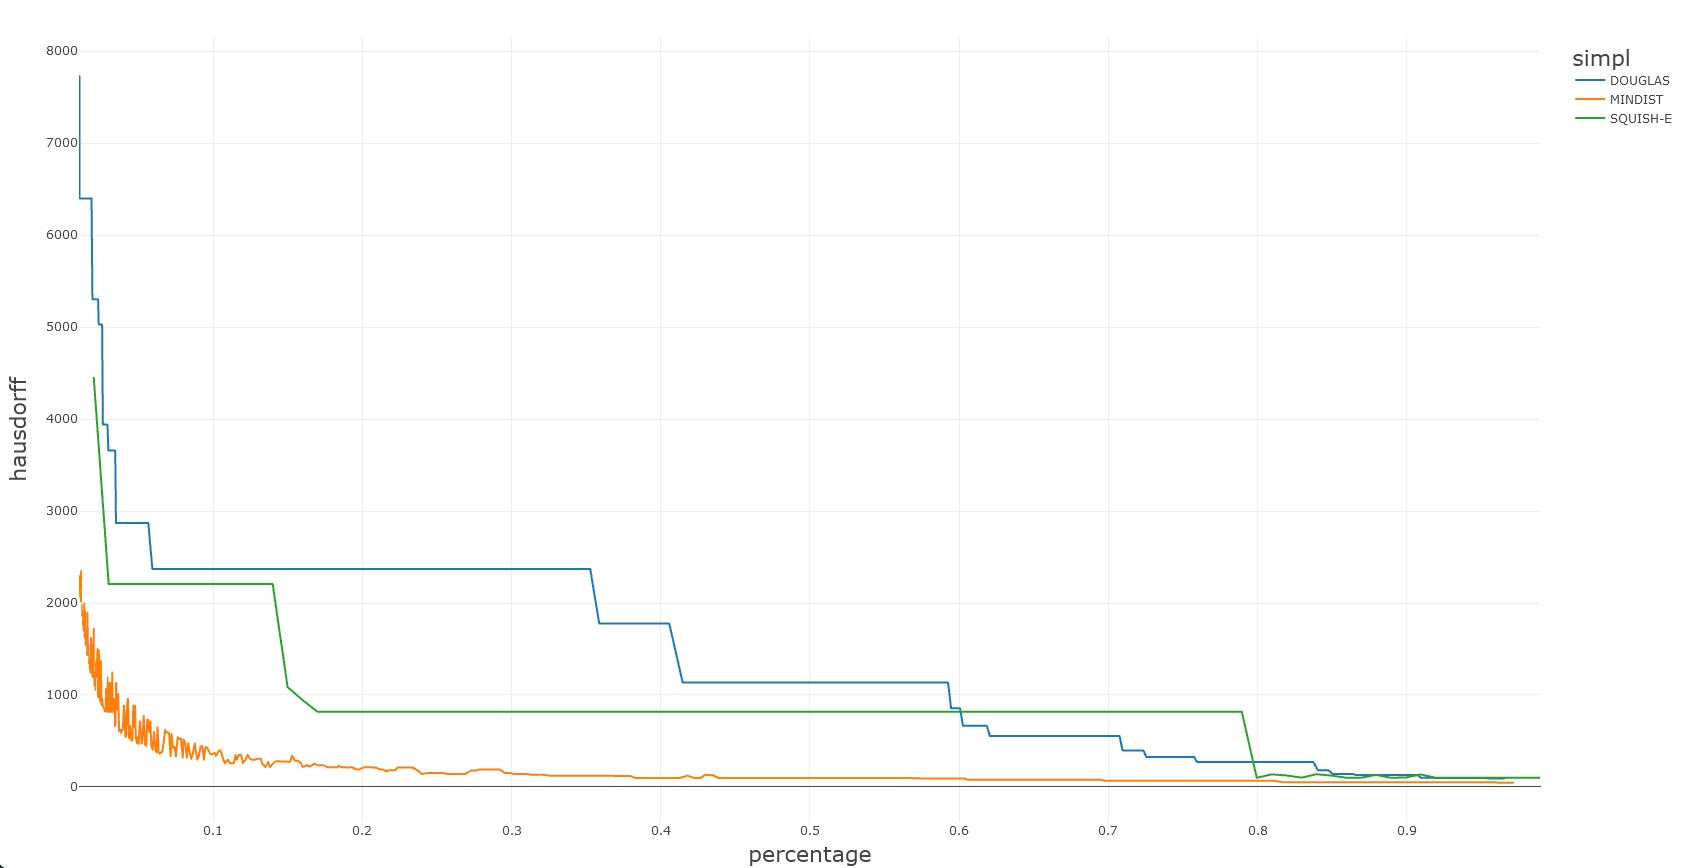
\includegraphics[width=1\linewidth]{figures/Stats/hausdorff_comp.jpg}
	\caption{Hausdorff comparison}
	\label{fig:comp_h}
\end{figure}


\begin{figure}[!h]
	\centering
	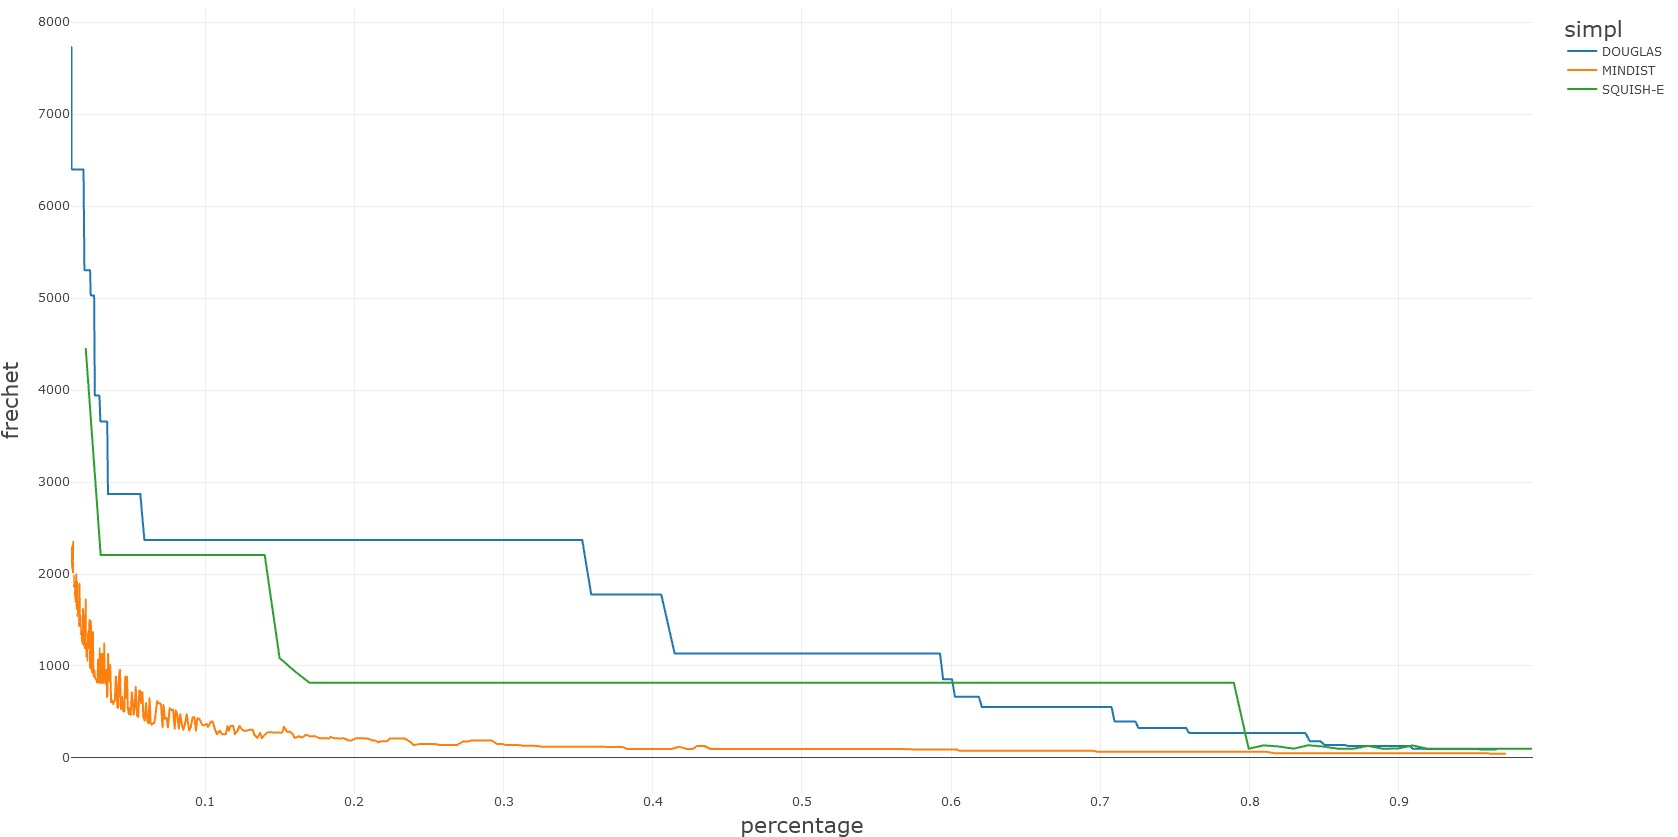
\includegraphics[width=1\linewidth]{figures/Stats/frechet_comp.jpg}
	\caption{Frechet comparison}
	\label{fig:comp_f}
\end{figure}


\begin{figure}[!h]
	\centering
	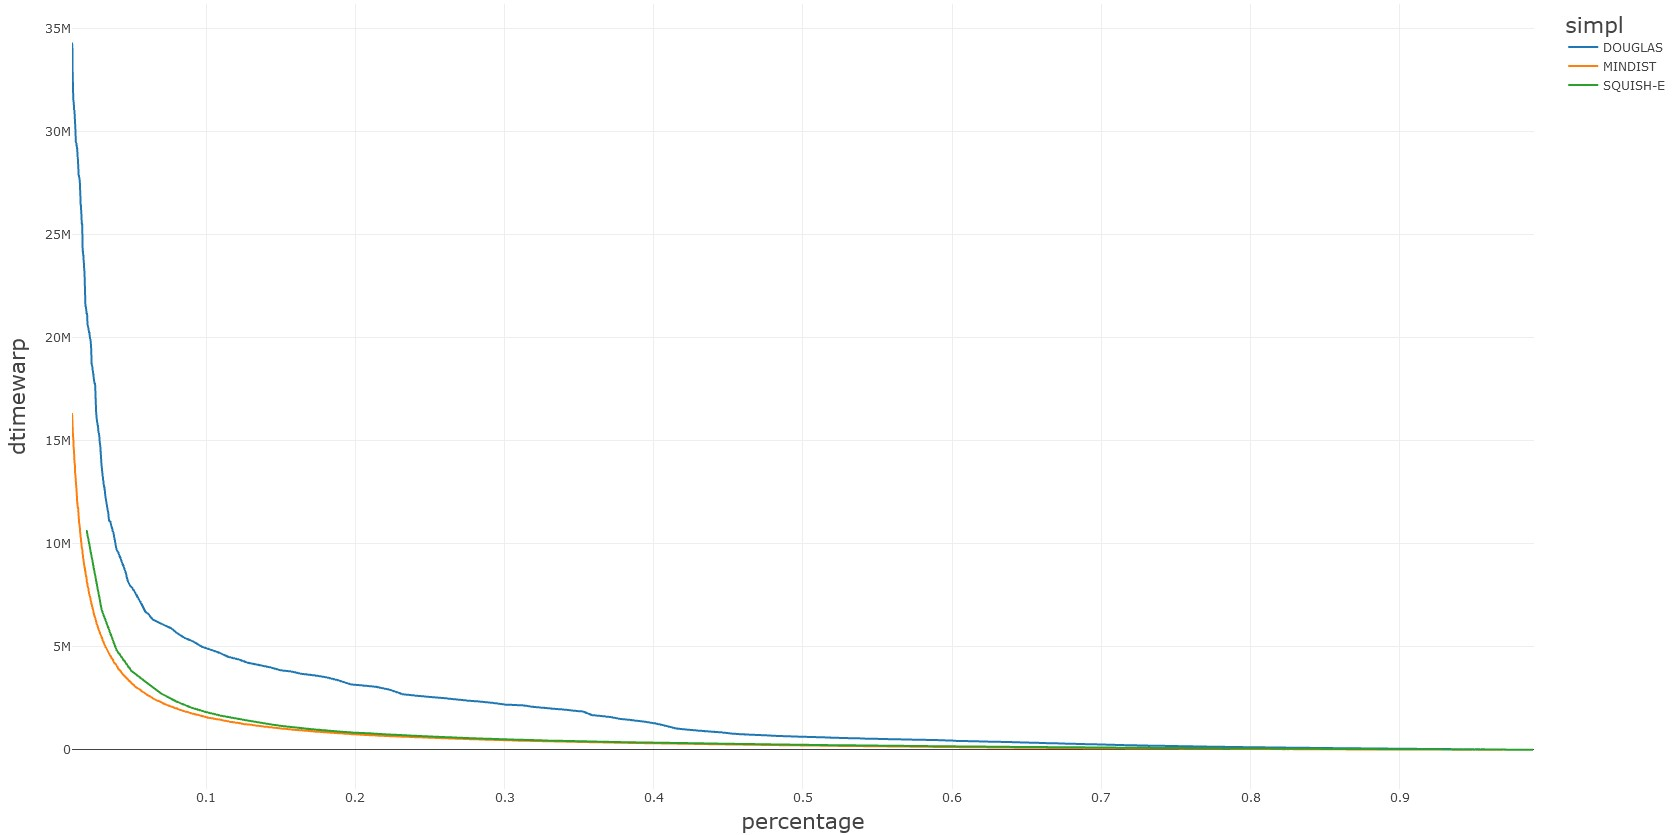
\includegraphics[width=1\linewidth]{figures/Stats/dtw_comp.jpg}
	\caption{DTW comparison}
	\label{fig:comp_dt}
\end{figure}


\begin{figure}[!h]
	\centering
	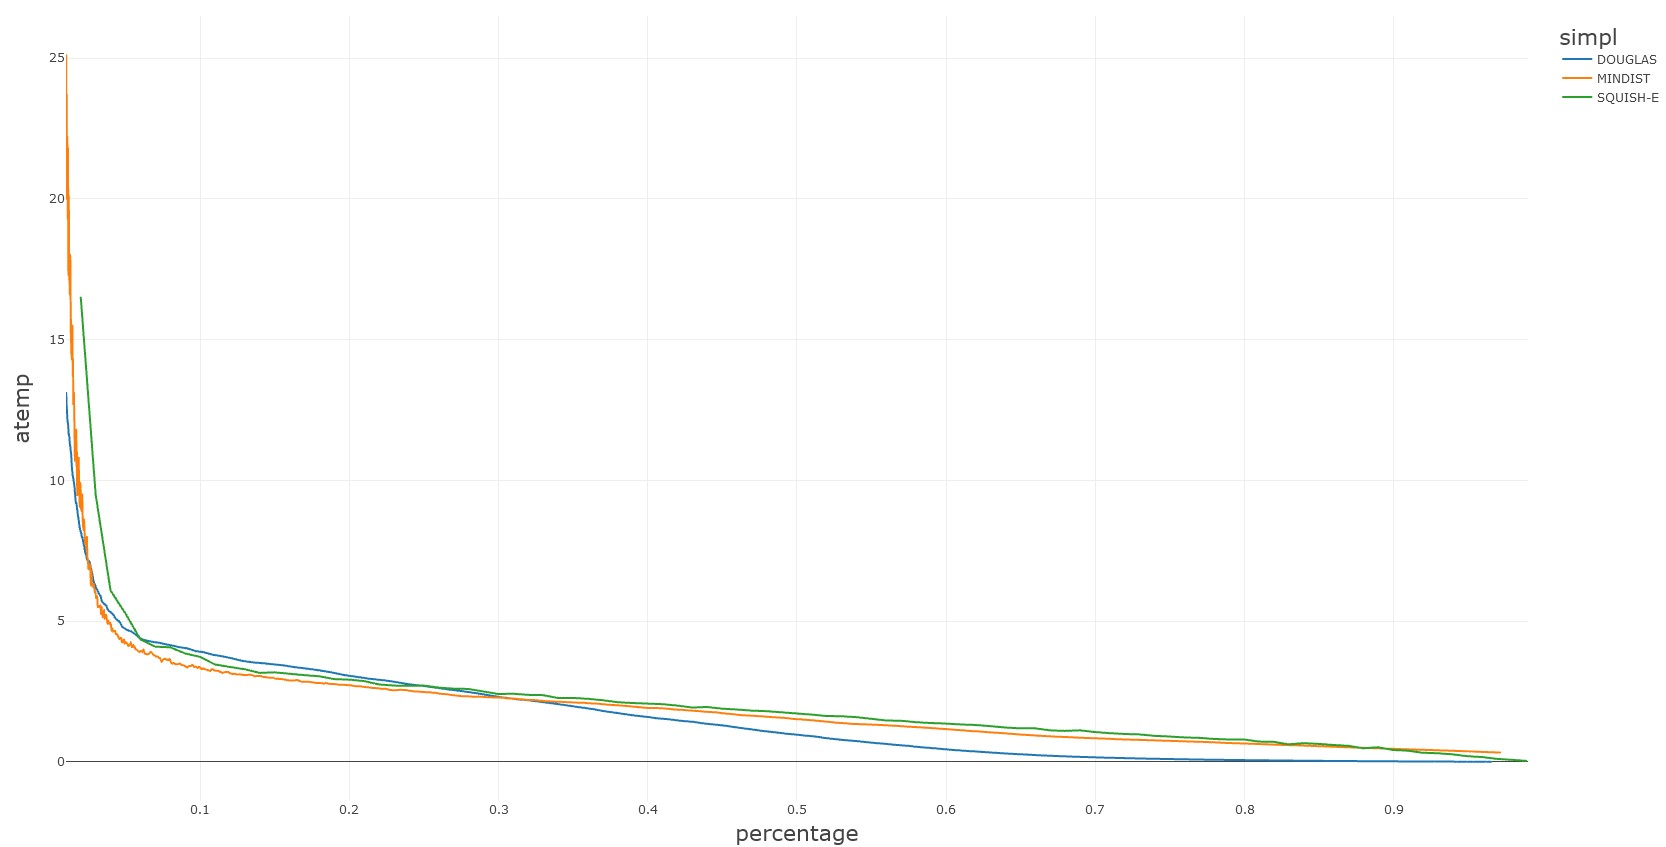
\includegraphics[width=1\linewidth]{figures/Stats/atemp_comp.jpg}
	\caption{Temporal Integral comparison}
	\label{fig:comp_at}
\end{figure}

These figures show the comparison of accuracies on trajectory 1 between the three algorithms mentioned above (Douglas,SQUISH-E,MinDist). Here the variation in error distance as a function of compression level can be observed. Frechet and Hausdorff's error level for Douglas and SQUISH-E has a staircase formation, while for Mindistance it constantly decreases. SQUISH-E is generally better than douglas and worse than min distance, except in \ref{fig:comp_at} where SQUISH-E is worse but very close to its competitors.


\chapter{Conclusion and Future Work}

In this thesis, at the beginning of the project, we addressed the issue of trajectory simplification and its realization in an online framework, so that it can be used as a node process in a streaming model. First and foremost, the state-of-the-art was analyzed in order to understand the various technologies and algorithms that address the problem. Then we selected a solution that corresponded to our expectations and analyzed it in order to understand it and to identify any possible challenges or problems linked to the algorithm. Next, we implemented the solution in a C code language that would enable it to be implemented in MobilityDB and also to be used as part of real-time processing by the technologies studied above. Next, we compared offline and online solutions to get an idea of the gap in simplification caused by streaming. Our observation is that the loss of accuracy between online and offline configuration is very small.  Lastly, there was a comparison with existing simplification algorithms on MobilityDB to get an idea of how the algorithm ranks against existing algorithms. SQUISH-E is a good candidate for solving the real-time simplification problem while maintaining a certain level of accuracy and performance. \\\\
First of all, we can look at different ways of comparing the accuracy of different trajectories. It's important to remember that the measurements and metrics used can be improved, and there are a huge number of metrics that could be useful, such as the variation in speed patterns between trajectories, or the volume of differences between two trajectories, as LIP does \cite{4438678}. It would therefore be a good idea to run and compare algorithms using different metrics to get an idea of their performance according to other criteria. Next we can note that the SQUISH-E algorithm has been modified during the process of this work to obtain a fully online algorithm. There are several possible improvements, starting with the choice of error function: in our case, SQUISH-E calculates its error distance using SED (synchronized euclidian distance), but it would be worth testing other error functions, or even inventing new ones, to see if it is possible to vary this parameter for use cases where other metrics become important, such as speed. As this work has not made any comparison between online algorithms, it is essential to compare online algorithms with each other and also to test them in real-life situations in order to obtain the perception of the reality gap between theory and practice. Finally, we'll see if we can improve implementation to reduce possible memory leaks, or code quality to make code more maintainable. All these ideas are part of the work produced and can be investigated.



\newpage
\printbibliography

\end{document}
